%			CLASS STYLE				%
\documentclass[prodmode,acmtecs]{acmsmall}

% Metadata Information
\acmVolume{12}
\acmNumber{3}
\acmArticle{1}
\articleSeq{1}
\acmYear{2013}
\acmMonth{5}

% Package to generate and customize Algorithm as per ACM style
\usepackage[ruled]{algorithm2e}
\renewcommand{\algorithmcfname}{ALGORITHM}
\SetAlFnt{\small}
\SetAlCapFnt{\small}
\SetAlCapNameFnt{\small}
\SetAlCapHSkip{0pt}
\IncMargin{-\parindent}

%		PACKAGES & MACROS		%
%\usepackage{graphics}
%\usepackage{epsfig}
%\usepackage{mathptmx}
\usepackage{amsmath}
\usepackage{amssymb} 
%\usepackage{listings}
%\usepackage{color}
%\usepackage{url}
\usepackage{graphicx}
%\usepackage{subfig}
%\usepackage{caption}
%\usepackage{algorithmic}
%\usepackage{algorithm2e}
%\usepackage{caption}
%\let\subcaption\undefined
%\usepackage{subcaption}
\usepackage{subfig}




% commands
\newcommand{\inlinecode}{\texttt}
\newcommand{\normal}{{\mathcal{N}}}
\renewcommand{\Re}{{\mathbb{R}}}
\newcommand{\R}{{\mathbb{R}}}
\newcommand{\Q}{{\mathbb{Q}}}
\newcommand{\Ze}{{\mathbb Z}}
\newcommand{\B}{{\mathbb B}}
\newcommand{\Ce}{{\mathbb C}}
\newcommand{\N}{{\mathbb{N}}}
\newcommand{\T}{{\mathbb T}}
\newcommand{\ie}{{\it i.e.}}
\newcommand{\eg}{{\it e.g.}}
\newcommand{\ea}{{\it et al }}
\renewcommand{\r}{\textcolor{red}}
\renewcommand{\b}{\textcolor{blue}}
\newcommand{\bk}{\textcolor{black}}
\newcommand{\argmin}{\textrm{arg}\min}
\newcommand{\Pre}{\mathrm{Pre}}
\def\transform{{\mathsf{filter}}}
\def\xduce{{\mathsf{xduce}}}
\def\set#1{{\{ #1 \}}}
\newcommand{\definedas}{\buildrel\triangle\over =}




%	HYPHENATION CORRECTION	%
\hyphenation{}

% Page heads
\markboth{P. Martin et al.}{Runtime Optimization of System Utility with Variable Hardware}

% Title portion
\title{Runtime Optimization of System Utility with Variable Hardware}
\author{PAUL MARTIN \affil{Electrical Engineering Department, University of California, Los Angeles} 
LUCAS WANNER \affil{Computer Science Department, University of California, Los Angeles}
MANI SRIVASTAVA \affil{Electrical Engineering Department,  University of California, Los Angeles}
}

% NOTE! Affiliations placed here should be for the institution where the
%       BULK of the research was done. If the author has gone to a new
%       institution, before publication, the (above) affiliation should NOT be changed.
%       The authors 'current' address may be given in the "Author's addresses:" block (below).
%       So for example, Mr. Fogarty, the bulk of the research was done at UIUC, and he is
%       currently affiliated with NASA.

%			ABSTRACT			%
\begin{abstract}
Increasing hardware variability in newer integrated circuit fabrication technologies has caused corresponding power variations on a large scale.  These variations are particularly exaggerated for idle power consumption, motivating the need to mitigate the effects of variability in systems whose operation is dominated by long idle states with periodic active states.  In systems where computation is severely limited by anemic energy reserves and where a long overall system lifetime is desired, maximizing the quality of a given application subject to these constraints is both challenging and an important step towards achieving high quality deployments.  This work describes VaRTOS, an architecture and corresponding set of operating system abstractions that provide explicit treatment of both idle and active power variations for tasks running in real time operating systems. Tasks in VaRTOS express elasticity by exposing individual \emph{knobs}---shared variables that the operating system can tune to adjust task quality and correspondingly task power, maximizing application utility both on a per-task and system-wide basis.  We provide results regarding online learning of instance-specific sleep power, active power, and task-level power expenditure on simulated hardware with demonstrated effects for several prototypical applications. Our results show that VaRTOS can reduce variability-induced energy expenditure errors from over 70\% in many cases to under 2\% in most cases and under 5\% in the worst-case. 
\end{abstract}

\category{D.4.7}{Operating Systems}{Organization and Design}[Real-time systems and embedded systems]
\category{D.4.1}{Operating Systems}{Process Management}[Threads]
\category{C.3}{Special-purpose and Application-Based Systems}{}[Real-time and embedded systems]

\terms{Design, Management, Performance}
\keywords{Variability, embedded operating systems, power consumption}

\acmformat{Paul Martin, Lucas Wanner, and Mani Srivastava. 2013. Runtime Optimization of System Utility with Variable Hardware.}
% At a minimum you need to supply the author names, year and a title.
% IMPORTANT:
% Full first names whenever they are known, surname last, followed by a period.
% In the case of two authors, 'and' is placed between them.
% In the case of three or more authors, the serial comma is used, that is, all author names
% except the last one but including the penultimate author's name are followed by a comma,
% and then 'and' is placed before the final author's name.
% If only first and middle initials are known, then each initial
% is followed by a period and they are separated by a space.
% The remaining information (journal title, volume, article number, date, etc.) is 'auto-generated'.

\begin{document}

\begin{bottomstuff}
This work is supported in part by the NSF under grants \# CCF-1029030, CNS-0905580,
CNS-0910706, and CNS-1143667\\
Author's address: P. Martin, Electrical Engineering Department, 420 Westwood Plaza, 56-125KK EEIV, Los Angeles,
C.A. 90095; email: pdmartin@ucla.edu; L. Wanner, Computer Science Department; email: wanner@ucla.edu; M. Srivastava, Electrical Engineering Department; email: mbs@ucla.edu
\end{bottomstuff}

\maketitle

%\addtolength{\abovedisplayskip}{-8pt}
%\addtolength{\belowdisplayskip}{-8pt}

%\setlength{\abovedisplayskip}{0pt}
%\setlength{\belowdisplayskip}{0pt}

%		INCLUDED SECTIONS		%
\section{Introduction}
The emergence of low power wireless systems in past decades was followed closely by attempts at optimizing energy efficiency and power consumption to facilitate long lifetime sensing deployments.  Research in this area was marked by many successes in the form of efficient time synchronization algorithms \r{cite?}, routing protocols \r{cite CTP?}, new sensing paradigms \r{cite CS?}, and the emergence of several widely-adopted operating systems for embedded systems (e.g., \cite{tinyos, contiki}). Newer IC fabrication technologies have introduced several additional variables into the energy management game; in addition to power variation across temperature, power variation on a per-instance level has become a non-trivial factor \cite{borkar2003, gupta2003}. Figure \ref{fig:variation} offers more intuition into the matter, showing the projected variation in idle and overall power as projected by IRTS for years to come \r{cite here} as well as recent variability results in the literature. 

Considerable research has focused on exposing energy and power measurements or estimates to the developer and even to the end user.  For example, techniques using linear combinations of instruction and performance counters \cite{sun2012,singh2009}, activity monitoring strategies \cite{appscope}, and various battery discharge-based models \cite{zhang2010} have been explored as tools for providing system-wide, application-specific, and even per-process granularities of energy usage.  Improved techniques for accurately  estimating and measuring power consumption will enable online power management in ways that were infeasible before, helping mitigate fabrication-induced per-instance chip variation as well \r{cite here?}. 

\begin{figure}
\centering
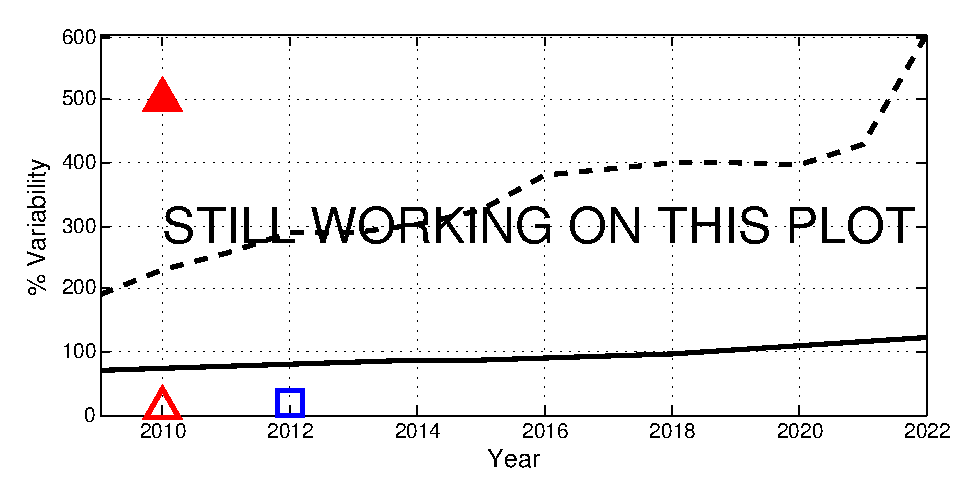
\includegraphics[width=1\columnwidth]{figures/projected_variations.eps}
\caption{\label{fig:variation}IRTS projections for sleep and idle power variability with measurements from recent literature.}
\end{figure}

Perhaps the most widely used and most effective strategies for extending the lifetime of energy-constrained systems are those based on controlling the ratio of active to idle time that the system is allowed, or \emph{duty cycling} a system.  Duty cycled systems take advantage of the disparity between active and idle power consumption, greatly increasing the lifetime of systems where latency and throughput constraints can be relaxed. Because of temperature and instance dependencies in power consumption, however, arriving at an optimal system-wide duty cycle ratio to achieve a lifetime goal given an energy constraint is difficult to do without emph{a priori} knowledge of instance-specific power models and temperature statistics for the target deployment location \cite{wanner2010}. Furthermore, applications involving more than one task introduce notions of fairness and utility---specifically, how should active processor time be distributed between each task so as to maximize the utility of the application and still meet the desired lifetime goal?

In this paper we explore the interplay between variable active and idle power consumption, deployment-specific temperature profiles, and multiple heterogeneous tasks with corresponding duty cycles. Specifically, we seek an answer to the question posed above; in an environment where power and temperature are measurable quantities, we seek an optimal strategy for distributing active processing time between arbitrary tasks so as to maximize application utility.  

Our contributions include the following: (1) we demonstrate an efficient and simple method for online-learning of idle and active power curves which are, in general, nonlinear functions of temperature; (2) we distill the minimum statistics regarding temperature required for accurate system lifetime predictions; (3) we evaluate VaRTOS, a series of kernel extensions to the FreeRTOS operating system that provides explicit treatment and online optimization of multiple-task duty cycles with corresponding utilities; and (4) we evaluate the effects of VaRTOS on several prototypical applications, using a modified version of the QEMU simulation suite \r{cite QEMU}.   



 % Paul
\section{Related Work}
\label{sec:relatedwork}

Hardware-level approaches to address variability have included statistical design approaches \cite{Neiroukh:2005,Datta:2005,Kang:2006}, post-silicon compensation and correction \cite{Gregg:2007,Khandelwal:2007,Tschanz:2002}, and variation avoidance~\cite{Choi:2004,Bhunia:2007,Ghosh:2007}. Furthermore, variation-aware adjustment of hardware parameters (e.g., voltage and frequency), whether in context of adaptive circuits (e.g., \cite{Borkar:2003,Ghosh:2007,Agarwal:2005}), adaptive micro architectures (e.g., \cite{Sylvester:2006,Ernst:2003,Meng:2006,Tiwari:2007}) or software-assisted hardware power management (e.g., \cite{Dighe:2010,Chandra:2009,Teodorescu:2008}) has been explored extensively in literature. 

While low-level treatment of hardware variation is a necessary step forward, application- and process-level adaptations have proven effective methods for combating variation.  The range of actions that software can take in response to variability includes:  altering the computational load by adjusting task activation; using a different set of hardware resources (e.g. using instructions that avoid a faulty module or minimize use of a power hungry module); changing software parameters (e.g., tuning software-controllable  variables such as voltage/frequency); and changing the code that performs a task, either by dynamic recompilation or through algorithmic choice.  Examples of variability-aware software include video codec adaptation~\cite{Pant:2011}, memory allocation~\cite{Bathen:2012}, procedure hopping~\cite{Rahimi:2012}, and error tolerant applications~\cite{Cho:2012}. In embedded sensing, \cite{matsuda2006} and \cite{garg2007} provide lifetime analyses for wireless sensor networks when considering variability power models, offering insights into what such systems stand to gain from explicit treatment of hardware variation.  Garg et al. estimated that a 37\% system lifetime improvement could be achieved through redundancy efforts that totaled a 20\% increased deployment cost. 

This work attempts to mitigate and exploit variations in power consumption through the management of elasticity in application quality by a variability-aware real-time scheduler.
Energy and longevity management in wireless sensor networks and low power embedded systems in general has long been an active area of research. Most previous work in this field, however, ignores the effects of power variations.
%Traditional power management techniques have assumed that, while idle and active powers vary as a function of temperature, they remain uniform across instances.  
Of these variability-agnostic techniques, many have focused on the tradeoff between energy and utility or performance.  For example, \cite{green2010,ghasemzadeh2012} represent attempts at making quality energy-proportional and tunable.  Specifically, \cite{green2010} introduces an architecture that allows developers to specify multiple versions of functions whereby the operating system can sacrifice quality when possible to reduce computational costs.  Similarly, \cite{ghasemzadeh2012} proposes tunable feature selection for wearable embedded systems, where less accurate feature computation can be used at the cost of inference quality. In real-time systems, \cite{liu1994} represents one of many efforts at using approximate computing to save energy where marginal losses in quality can be afforded. In ECOSystem~\cite{Zeng:2002} and Cinder~\cite{Rumble:2009}, energy resources are periodically distributed to tasks which must spend the resources to perform system calls. In these systems, applications adjust their computational load according to energy availability. Our work differs from the previous approaches in that applications need not manage energy directly but instead expose their elasticity in the form of a variable knob that is controlled by the operating system scheduler. Power consumption characteristics for each individual sensor are learned over time, and the system maximizes quality of service across tasks in a variability-aware fashion. 




This work is closely related to that of \cite{Wanner:2012}.  There, the authors describe a method for calculating a system-wide optimal duty cycle ratio given known models for active and idle power as well as probability density functions for deployment temperatures. Here we provide an extension to the work in \cite{Wanner:2012}, showing methods for online learning of power models and providing notions of utility in multi-task applications.  


 % Lucas
\section{Power Variability}

As fabrication technologies improve and feature sizes decrease, hardware variation plays an increasingly important role in determine the power consumption and therefore lifetime of computer systems.  While the large baseline in active power consumption relative to idle power consumption amortizes these variations to some degree (\cite{wanner2011} cites a 10\% variation in active power while \cite{balaji2012} cites between 7\% and 17\% variation), the low baseline in idle power consumption renders it highly susceptible to fabrication-induced variations (\cite{wanner2011} reports a 14x range in measured idle powers across 10 instances of ARM Cortex M3 processors). 

Power consumption in energy-constrained embedded systems is often dominated by time spent in an idle state, waiting to sense, communicate, or perform a processing task. Consequently, the lifetimes of these systems can be wildly variant due to instance-to-instance variation in idle power.  The result of inaccurate lifetime estimates obtained by improper power models can be one of two things: conservative designs can make sure that lifetime is met by adding a guard band to system duty cycle and thus underperforming, or removing these guard bands will result in higher performance while all subsystems (perhaps nodes in a network) are still running, but upon depletion of energy reserves by those processors with higher power consumption the entire system will again suffer.  A processor-specific duty cycle can be assigned so that all lifetimes are met, but without a strategy for distributing resources to individual tasks on a processor there is no guarantee that these variations are handled elegantly and in a way that maximizes application utility. % Lucas
\section{Optimizing Utility with Variable Hardware}
\label{sec:optimization}

One way to combat increasing power variability is for an application to decrease or increase quality, thereby decreasing or increasing energy consumption.  In this section we explore an architecture for adapting quality when applications have some degree of elasticity---that is, when quality is not a hard constraint.   This will be accomplished by introducing task \emph{knobs}---task-specific expressions of quality and power elasticity. 

\subsection{Task Modeling}
We start first by introducing an application as a set of $N$ {tasks} denoted $\tau_i,~i = 1,\ldots,N$, where each task represents a periodic application subprocess.  We associate with each task and with the application as a whole a utility $u_i$ (or $u_{sys}$ for the entire application) with the understanding that utility represents some notion of quality that the user is interested in. 
While some efforts espouse an architecture wherein each $u_i$ is defined by an arbitrary function (\cite{green2010} for example), we advocate a simplified model where the OS constructs $u_i$ based on a few key inputs from the developer.  In doing so, we assume that $u_i$ is a monotonically non-decreasing function of the active computational time for $\tau_i$ denoted $t_{a,i}$ or, equivalently, the duty cycle ratio specific to $\tau_i$ denoted $d_i$ and defined as $d_i = t_{a,i}/(t_{a,i} + t_{s,i})$ where $t_{s,i}$ is the amount of time that $\tau_i$ is inactive. These variables along with additional key variables used throughout the text are summarized in Table \ref{tab:vars}.\\

\noindent\emph{\underline{Task Knobs}}: 
In order to tune the active time used per task and thus the task-specific duty cycle ratio $d_i$, we introduce the notion of task knobs.  In practical terms, a task knob is a variable that will govern either (1) the period of a task or (2) the frequency with which a task is activated. We argue that a large portion of tasks found in embedded applications will fall in one of these two classes, and those that require both frequency and period modulation can often be divided into two legal subtasks coupled with inter-process communications. For example, tasks that fall under class 1 include variable length sensing tasks, tasks that listen for inbound communication, and variable length processing chains.  Those that fall under class 2 include variable frequency transmission, variable frequency sensor sampling, time synchronization handshaking, control and actuation events, and more.  

We define task knobs, denoted $k_i$, such that increasing $k_i$ will increase $t_{a,i}$, $d_i$, and consequently $u_i$.  Task knobs are created by passing a variable address to the OS, allowing direct manipulation of knob values by an optimization routine.  In addition, the developer specifies a minimum and maximum knob value, $k_{i,min}$ and $k_{i,max}$. The value $k_{i,min}$ specifies the minimum value of $k_i$ that yields a nonzero utility.  Below this value, a task offers no utility.  The value $k_{i,max}$ specifies a value after which increasing $k_i$ further will yield  no added utility.  \\
%As an example, a radio transmission task may be useless if it does not meet a certain latency requirement, but usefulness may plateau at some frequency governed perhaps by the physics and time response of the event being sensed.\\

\noindent\emph{\underline{Generating Utility Curves}}: Changing each knob value $k_i$ will cause a corresponding change in duty cycle ratio $d_i$ based on the nature of $\tau_i$.  Given $k_{i,min}$ and $k_{i,max}$ as well as a mapping from $k_i$ to $d_i$ (to be discussed later) we can construct a utility function $u_i = f(d_i)$ as a modified logistic (Sigmoid) function of the form $f(d_i) = {1\over{1 + e^{-c_id_i}}}, ~c_i \ge 0$.  A logistic function is used because the convex portion of the characteristic \emph{s}-like curve offers a convenient form for modeling diminishing returns on $k_i$.   The convex portion of the logistic function can be isolated by choosing $u_i$ to be of the particular form

\begin{equation}
\label{eq:util}
u_i(d_i) = { 2\over { 1 + e^{-c_id_i }} }- 1, ~~c_i \ge 0, ~~d_{i,min} \le d_i \le d_{i,max}
\end{equation}

where $d_{i,min}$ and $d_{i,max}$ are task duty cycles corresponding to $k_{i,min}$ and $k_{i,max}$.  Here, $c_i$ governs the convergence rate of $u_i$ from the minimum utility to the maximum utility and is calculated as a function of $k_{i,min}$ and $k_{i,max}$ such that 99\% of the utility has been reached by $k_{max}$.  Increasing the percentage of $u_{i,max}$ realized by $k_{i,max}$ has the effect of steepening the utility curve and thus increasing the rate at which returns diminish. The constant $c_i$ can be calculated from Equation \ref{eq:util} by enforcing $u_i(d_{i,max}) - u_i(d_{i,min})$ to be $\epsilon = 0.99$ as shown below:

\begin{equation}
c_i = { -\log\left( {2\over \epsilon + 1} - 1 \right) \over (d_{i,max} - d_{i,min}) }, ~~~~\epsilon = 0.99
\end{equation}

\begin{figure*}[t]
\centering
{\centering
\begin{minipage}{0.47\textwidth}
  \centering

\captionof{table}{\label{tab:vars}Summary of selected variables}
\centering
\begin{tabular}{c|c}
\hline
Variable name & Definition \\ \hline
$\tau_i$ & Task $i,~~i = 1,\ldots,N$ \\
$t_{a,i}$ & Active time for $\tau_i$ \\
$t_{s,i}$ & Inactive time for $\tau_i$ \\
$d_i$ & D.C. ratio for $\tau_i$ \\
$\pmb{d}$ & the vector $[d_1 \cdots d_N]$ \\
$d_{sys}$ & System-wide D.C. \\
$k_i$ & Knob value for $\tau_i$ \\
$\pmb{k}$ & the vector $[k_1 \cdots k_N]$ \\
$\mathcal{K}_i$ & model of $k_i \rightarrow d_i$ \\
$u_i$ & utility fcn. for $\tau_i$ \\
$p_i$ & priority scalar for $\tau_i$ \\
$E$ & energy budget \\
$L$ & desired lifetime \\ \hline
\end{tabular}

\end{minipage}
\hspace{.04\textwidth}
\begin{minipage}{0.47\textwidth}
  \centering
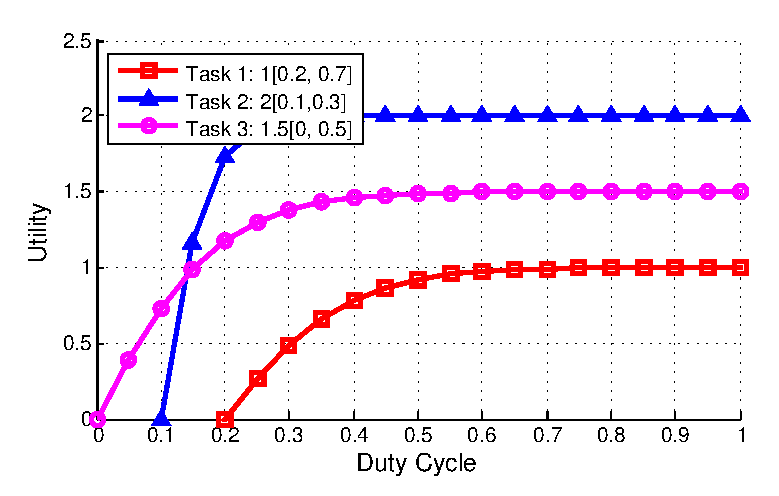
\includegraphics[width=\textwidth]{figures/utilityfunctions}
  \captionof{figure}{\label{fig:util}Example utility curves. Task 1 has priority scalar $p_1 =  1$ with useful range $d_1 = [0.2, 0.7]$, task 2 with $p_2 = 2$ and $d_2 = [0.1, 0.3]$, and finally task 3 with $p_3 = 1.5$ and $d_3 = [0, 0.5]$.}
\end{minipage}
}
\end{figure*}

Finally, each utility curve can be arbitrarily increased or decreased by a priority scalar $p_i \in \R^+$ for tasks with intrinsically higher or lower utility than others.  This offers a level of customizability in addition to specifying $k_{i,min}$ and $k_{i,max}$, allowing the developer to give preference to one task over another. Figure \ref{fig:util} shows three example utility curves corresponding to three tasks with various priorities and duty cycle ranges (resulting from various $k_{i,min}$ and $k_{i,max}$). \\

\noindent\emph{\underline{Learning $\mathcal{K}_i$, the $k_i \rightarrow d_{i}$ Relation}}: Because the developer has free reign to use the knob $k_i$ for each task as desired, the function mapping $k_i$ to active time $t_{a,i}$ and thus $d_i$ is not known \emph{a priori}. Instead, the transformation $\mathcal{K}_i$ that maps $k_i$ to $d_{i}$  is assumed linear and is learned through regression at runtime. Should the developer misuse $k_i$ in a way that is nonlinear or that results in non-increasing values of $t_{a,i}$, the linear model will introduce errors that will affect the optimization process. Dividing active time accumulated per task by a fixed supervisory time interval $t_{super}$ yields task-specific duty cycle ratios, $d_i$. 


\subsection{Maximizing Application Utility}
\label{sec:optimization:maxutil}
Given the set of tasks $\{\tau_1,\ldots, \tau_N\}$, our ultimate goal is to optimize $u_{sys} = \sum_{i=1}^Nu_i$, the overall system utility. That is, we seek a solution to the convex optimization problem

\begin{equation}
\label{eq:linprog_util}
u_{sys}^* = \max_{\pmb{k}} \sum_{i=1}^N{ 2\over { 1 + e^{-c_i\mathcal{K}_i[k_i] }} }- 1,
\end{equation}
\begin{align*}
\text{subject to:~~~~} \sum_{T=T_{min}}^{T_{max}}f_T\mathcal{L}[\pmb{k}] \le { E \over L} = \bar{P} \\ 
\end{align*}

Where $T_{min}$ and $T_{max}$ are the minimum and maximum temperatures for a given location, $\pmb{k} = [k_1 ~\cdots~ k_N]$ is the vector of task knobs, and $\mathcal{L}$  is a linear mapping from $\pmb{k}$ to power consumption.  The parameters $E$ and $L$ are the energy budget and desired lifetime as specified by the user and resulting in an average power goal, $\bar{P}$. In general, $\mathcal{L}$ is a function of temperature, and thus summing over the range of temperatures $[T_{min}~~T_{max}]$ and scaling by the probability density of each temperature $f_T$ gives the predicted power consumption corresponding to the knob vector $\pmb{k}$. When using external peripherals (such as radios, analog to digital converters, and flash storage), $\mathcal{L}$ incorporates both external power and internal power (i.e., power consumed by the processor).  In the remainder of this paper, we will focus on optimizing utility when $\mathcal{L}$ includes the power consumption of the processor alone.  We leave inclusion of peripheral power models as a natural and straightforward extension to the proposed architecture. 

We shift our focus now from that of optimizing utility with a power constraint to that of optimizing utility with a duty cycle constraint.  In other words, power consumption of the system as a whole can take on values in the range $[P_s(T) ~~P_a(T)]$ for a given temperature $T$ dictated by the overall system duty cycle ratio, $d_{sys} = \sum_{i=1}^Nd_i$: $P = (1-d_{sys})P_s + d_{sys}P_a$. Again, both $P_s$ and $P_a$ are functions of temperature so that, replacing $\mathcal{L}$ with the processor power models, the optimization problem becomes

\begin{equation}
\label{eq:linprog_dc}
u_{sys}^* = \max_{\pmb{d}} \sum_{i=1}^N{ 2\over { 1 + e^{-c_id_i }} }- 1,
\end{equation}
\begin{align*}
\text{subject to:~~~~} &\sum_{T=T_{min}}^{T_{max}}f_T\left[\sum_{i=1}^N\left( d_iP_a(T) + (1-d_i)P_s(T)\right)\right] \le {E\over L} = \bar{P} \\ 
\end{align*}

Here we have replaced the knob vector $\pmb{k}$ with the duty cycle vector $\pmb{d}$ similarly defined.  The system-wide duty cycle can be arrived at if we know \emph{a priori} the future environmental temperatures, the function mapping temperature to sleep power $P_s$, and the function mapping temperature to active power $P_a$. Given these, the optimal (maximum)  duty cycle $d_{sys}^* \in [0,1]$ follows naturally from Equation \ref{eq:linprog_dc}: 

\begin{equation}
\label{eq:linprog_fin}
d_{sys}^* = \max ~{d}~~
\end{equation}
\begin{align*}
\text{subject to:~~~~}  \sum_Tf_T\left[dP_a(T) + (1-d)P_s(T)\right] \le {E\over L} = \bar{P}
\end{align*}

%Arriving at $d^*$ is done in the same way as set forth in \cite{Wanner:2012} with the exception that the active and idle/sleep powers ($P_a$ and $P_s$) are learned at runtime.  

Under practical conditions as outlined in \cite{Wanner:2012}, a close approximation for the optimal solution to Equation \ref{eq:linprog_fin} can be obtained algebraically using Equation \ref{eq:dstar}, where we have introduced the temperature-averaged power quantities $\bar{P_s}$ and $\bar{P_a}$:

\begin{equation}
\label{eq:dstar}
d_{sys}^* =  { E - L\bar{P_s} \over L(\bar{P_a} -\bar{P_s}) } 
\end{equation}


\begin{figure*}[t]
\centering
{\centering
\begin{minipage}{0.47\textwidth}
  \centering
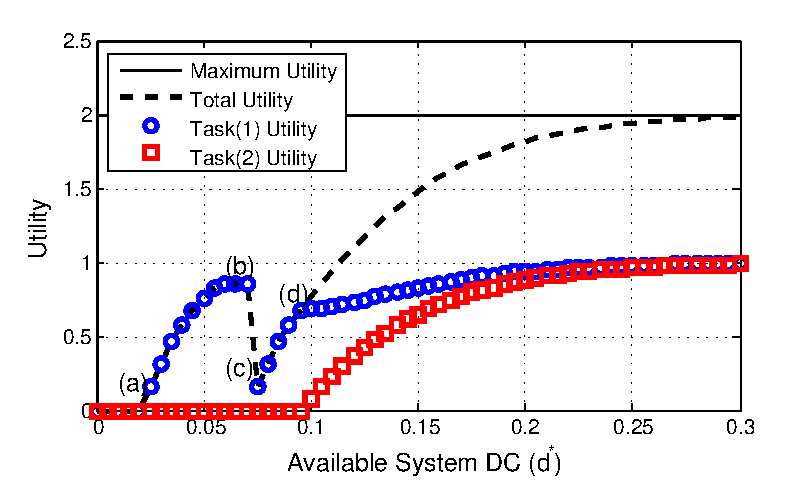
\includegraphics[width=\textwidth]{figures/optimalDCexample}
  \captionof{figure}{\label{fig:optimaldc_mult}Maximizing utility for two tasks and different values of system duty cycle, $d_{sys}^*$}
\end{minipage}
\hspace{.04\textwidth}
\begin{minipage}{0.47\textwidth}
  \centering
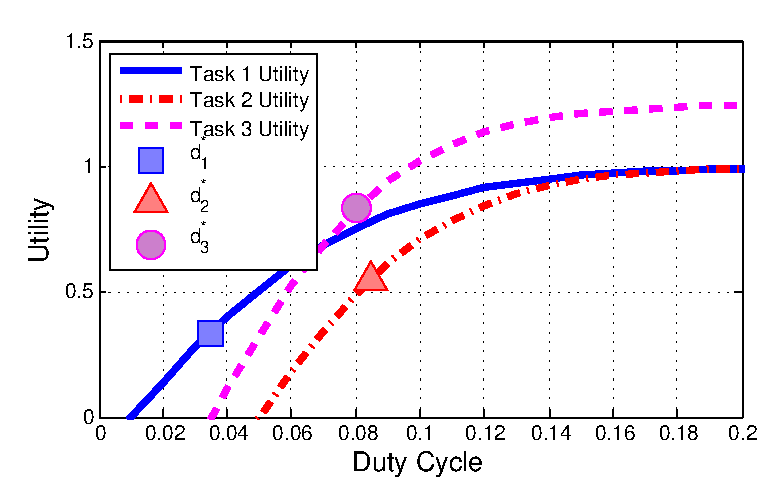
\includegraphics[width=\textwidth]{figures/utilanddc}
  \captionof{figure}{\label{fig:utilanddc}Example optimal duty cycle points for 3 example tasks with different values for $\{k_{min},k_{max}, p_i\}$}
\end{minipage}
}
\end{figure*}

Given $d_{sys}^*$, we now seek an efficient solution to Equation \ref{eq:linprog_dc}.  Because we have chosen $u_i$ to be a logistic function, we can use a greedy approach when optimizing utility.  The optimization routine will be a two step process: (1) attempt to assign the minimum duty cycle $d_{i,min} = \mathcal{K}_i[k_{i,min}]$ needed for each task in order of decreasing priority, and (2) continue distributing computational time in small increments to those tasks yielding the largest marginal utility until no active computational time is left. This process is outlined in Algorithm \ref{alg}. Duty cycle is incrementally added by a small fraction $\delta$ (chosen sufficiently small to ensure accuracy) to those tasks with the largest marginal utility defined as 

\begin{equation}
max\_mu = \max\{mu_1,\ldots,mu_N\},~~~ mu_i = { u_i[d_i+\delta] - u_i[d_i]   \over \delta }
\end{equation}

until $d_{sys}^*$ as calculated from Equation \ref{eq:dstar} is exhausted. Figure \ref{fig:optimaldc_mult} shows an example of the utility maximization algorithm for two example tasks with the total system duty cycle on the $x$-axis and utility on the $y$-axis. .  At point (a), $k_{1,min}$ is met and task 1 begins to receive active time.  At point (b), task 1 begins to plateau as $mu_1$ diminishes.  At point (c), both $k_{1,min}$ and $k_{2,min}$ can be met; starting with task 1 with the highest $mu$, utility is increased until point (d) where task 2 and 1 go back and forth bidding for active time.  The dashed curve illustrates the total system utility, $u_{sys} = u_1 + u_2$. 

% Algorithm
\begin{algorithm}[t]
\SetAlgoNoLine
\KwIn{System duty cycle, $d_{sys}^*$, linear functions $\{\mathcal{K}_1,\ldots,\mathcal{K}_N \}$, and utility curves $\{u_1,\ldots,u_N\}$ }
\KwOut{The optimal task duty cycles $\pmb{d}^* = \{d_1^*,\ldots,d_N^*\}$}
$\pmb{\tau} \leftarrow \text{sort}(\{\tau_1,\ldots,\tau_N\})$ by decreasing $p_i$\\
$d_{remaining} \leftarrow d_{sys}^*$.  \\
//{ Assign minimum knob values for tasks that can be scheduled:}\\
$\pmb{\tau}_{scheduled} \leftarrow \{~\}$ // empty set \\
 \For{$i \in \pmb{\tau}$}{
 	\eIf{$\mathcal{K}_i[k_{i,min}] < d_{remaining}$}{
 	$d_i = \mathcal{K}_i[k_{i,min}]$\\
	$d_{remaining} \leftarrow d_{remaining} - d_i$ \\
	append $\tau_i$ to  $\pmb{\tau}_{scheduled}$
 	}{
 	stop
 	}
 }
 // Allocate remaining duty cycle fairly:\\
 \While{$d_{remaining} > 0$}{
 	// Find highest marginal utility $max\_mu$ and the set $\pmb{\tau}_{max}$ of tasks yielding $max\_mu$:\\
	$[max\_mu, \pmb{\tau}_{max}] \leftarrow$ Find Maximum Marginal Utility$(\pmb{\tau}_{scheduled})$\\
	 $d_{requested} \leftarrow \min\{ \delta \cdot |\pmb{\tau}_{max}|, ~d_{remaining} \}$\\
	 \For{$i \in \pmb{\tau}_{max}$}{
		$d_i \leftarrow d_i + {1\over |\pmb{\tau}_{max}|}d_{requested}$
	 }
 }
$\pmb{d}^* \leftarrow \{d_1,\ldots, d_N\}$
\caption{\label{alg}Greedy Utility Optimization}
\label{alg:one}
\end{algorithm}

Each point in Figure \ref{fig:optimaldc_mult} represents a different environmental set up---that is, a different $d_{sys}^*$ ($x$-axis) resulting from, perhaps, different values for $E$, $L$, and $\pmb{f}_T$. At each $d_{sys}^*$, all tasks are assigned a specific duty cycle ratio $d_i$.  For example, Figure \ref{fig:utilanddc} shows the resulting duty cycles $\{d_1, d_2, d_3\}$ for three tasks when $d_{sys}^* = 0.2$.  The vector $\pmb{d}$ that maximizes Equation \ref{eq:linprog_dc} is denoted $\pmb{d}^* = \{d_1^*,\ldots,d_N^*\}$. 

With a method in hand to calculate an optimal $d_{sys}^*$ offline, we seek a method for both calculating $d_{sys}^*$ and achieving $d_i \in \{d_1,\ldots,d_N\}$ in an efficient, online manner.  Our implementation of this architecture is called VaRTOS and is the subject of the following section. 



 % Paul
\section{VaRTOS, the Variability Aware Real Time Operating System}
\label{sec:vartos}

In this section we outline the implementation of the architecture and algorithms presented in Section \ref{sec:optimization} as a series of extensions to an existing real time operating system (RTOS).  The results shown are using a modified version of the FreeRTOS operating system \cite{freertos}, though the architecture is easily applied to other embedded operating systems as well. The design of VaRTOS must accomplish several key aspects of Section \ref{sec:optimization} while remaining lightweight and energy-efficient.  In particular, VaRTOS includes the following functionality: (1) a method for online modeling of $P_s(T)$ and $P_a(T)$; (2) a method for online modeling of $\mathcal{K}_i$; (3) OS-level control over task knobs $\{k_1,\ldots,k_N\}$; and (4) a tool for evaluating the effects of user inputs $\{k_{i,min},k_{i,max},p_i,E,L\}$ as well as deployment location (temperature profile).  We will describe each of these subsystems in detail below, with various prototypical case studies discussed in Section \ref{sec:casestudies}. 

% Power learning figure
\begin{figure*}
\centering
\subfloat[]{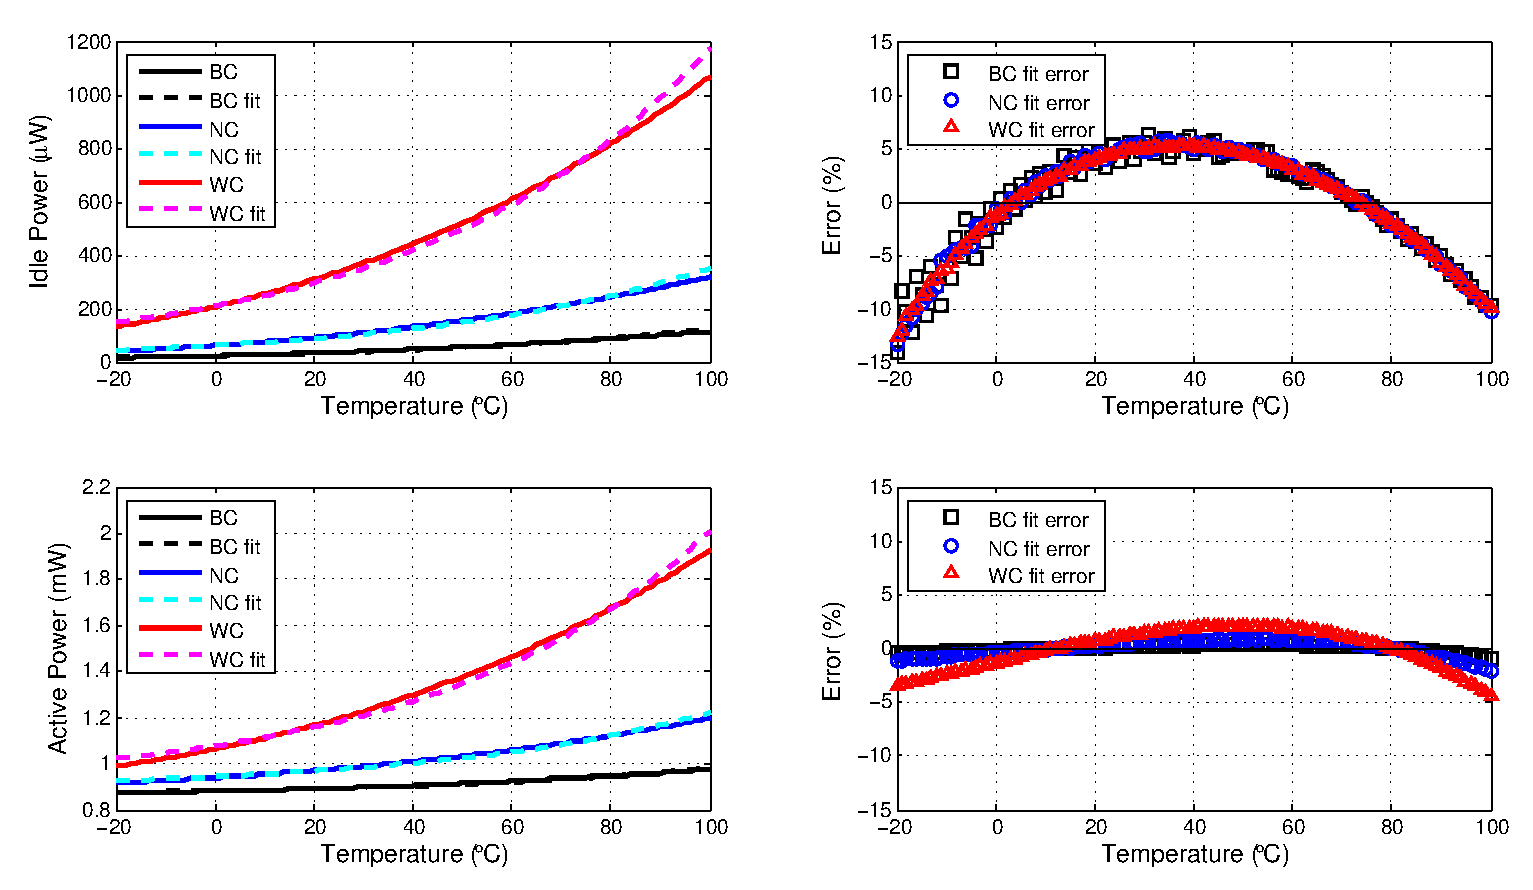
\includegraphics[width=0.47\textwidth, clip=true, trim=0 2.855in 5in 0in]{figures/powerlearning}}
\subfloat[]{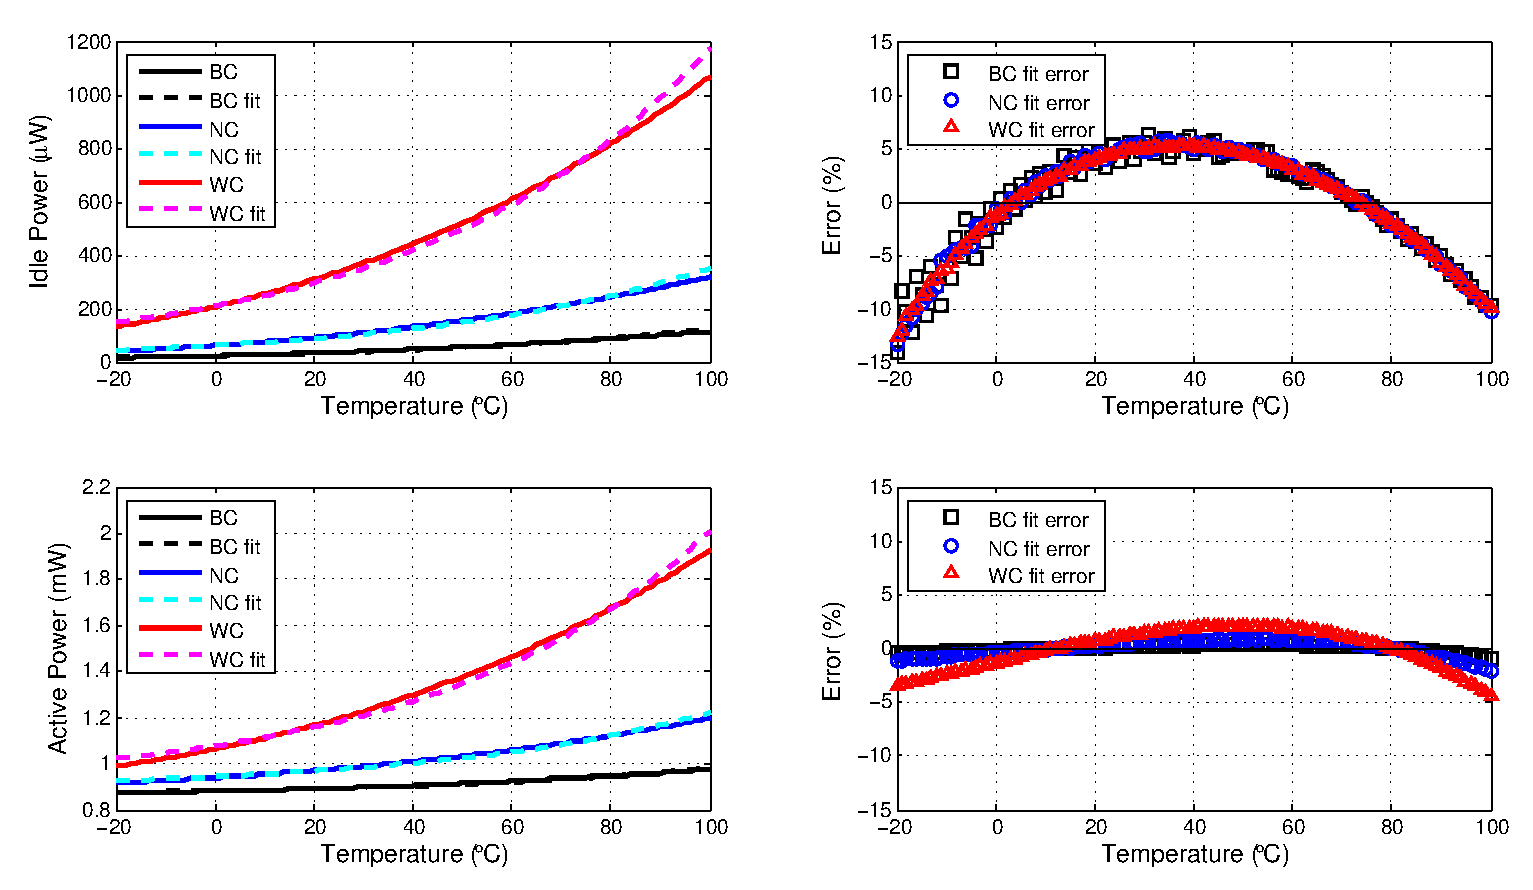
\includegraphics[width=0.47\textwidth, clip=true, trim=5in 2.855in 0in 0in]{figures/powerlearning}}\\
\subfloat[]{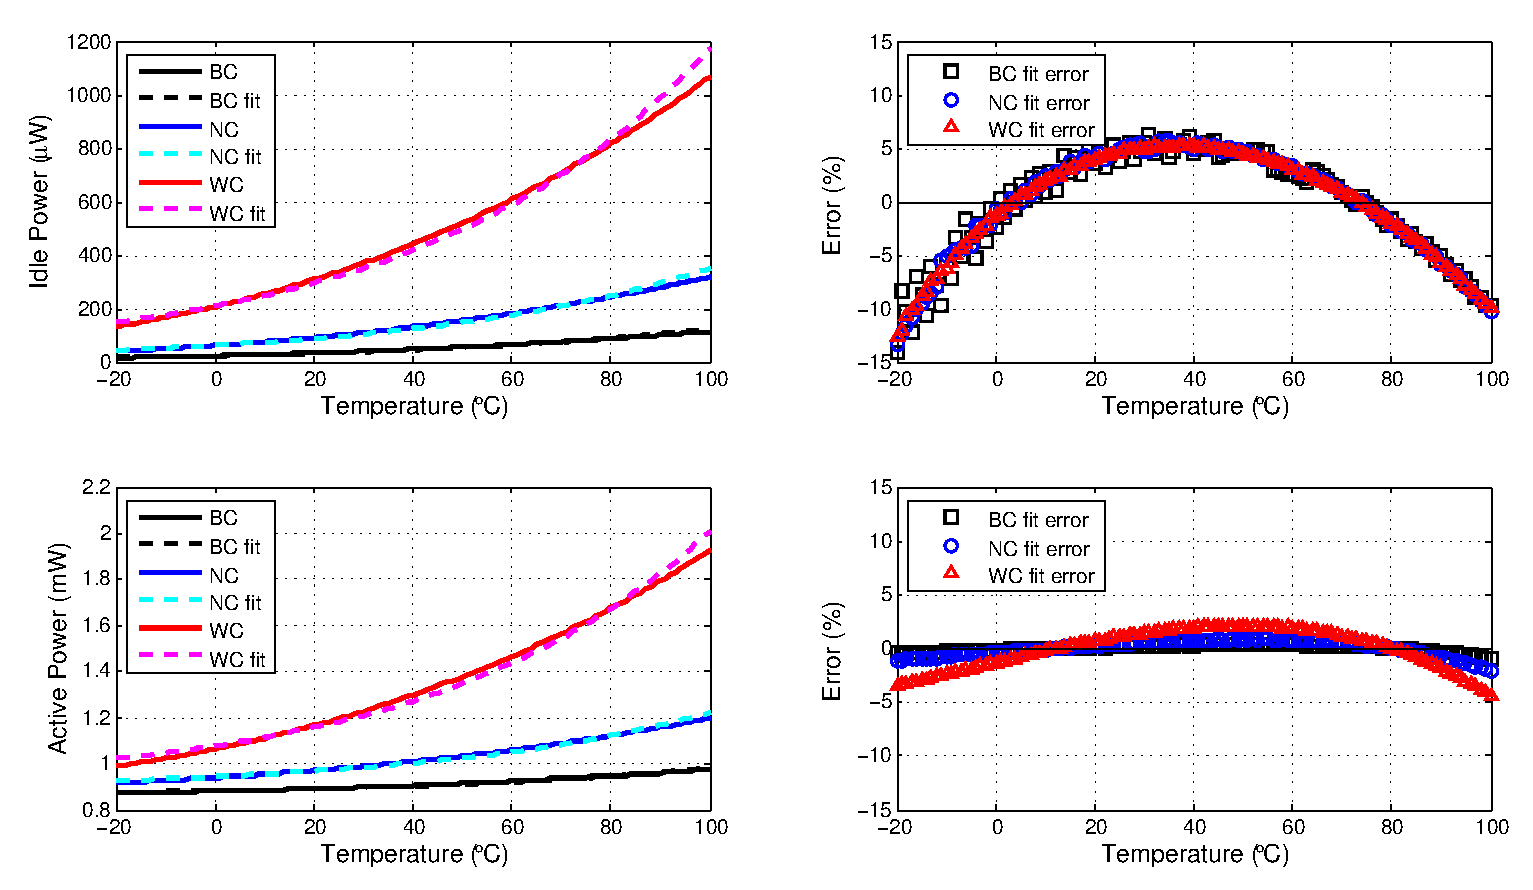
\includegraphics[width=0.47\textwidth, clip=true, trim=0in 0in 5in 2.855in]{figures/powerlearning}}
\subfloat[]{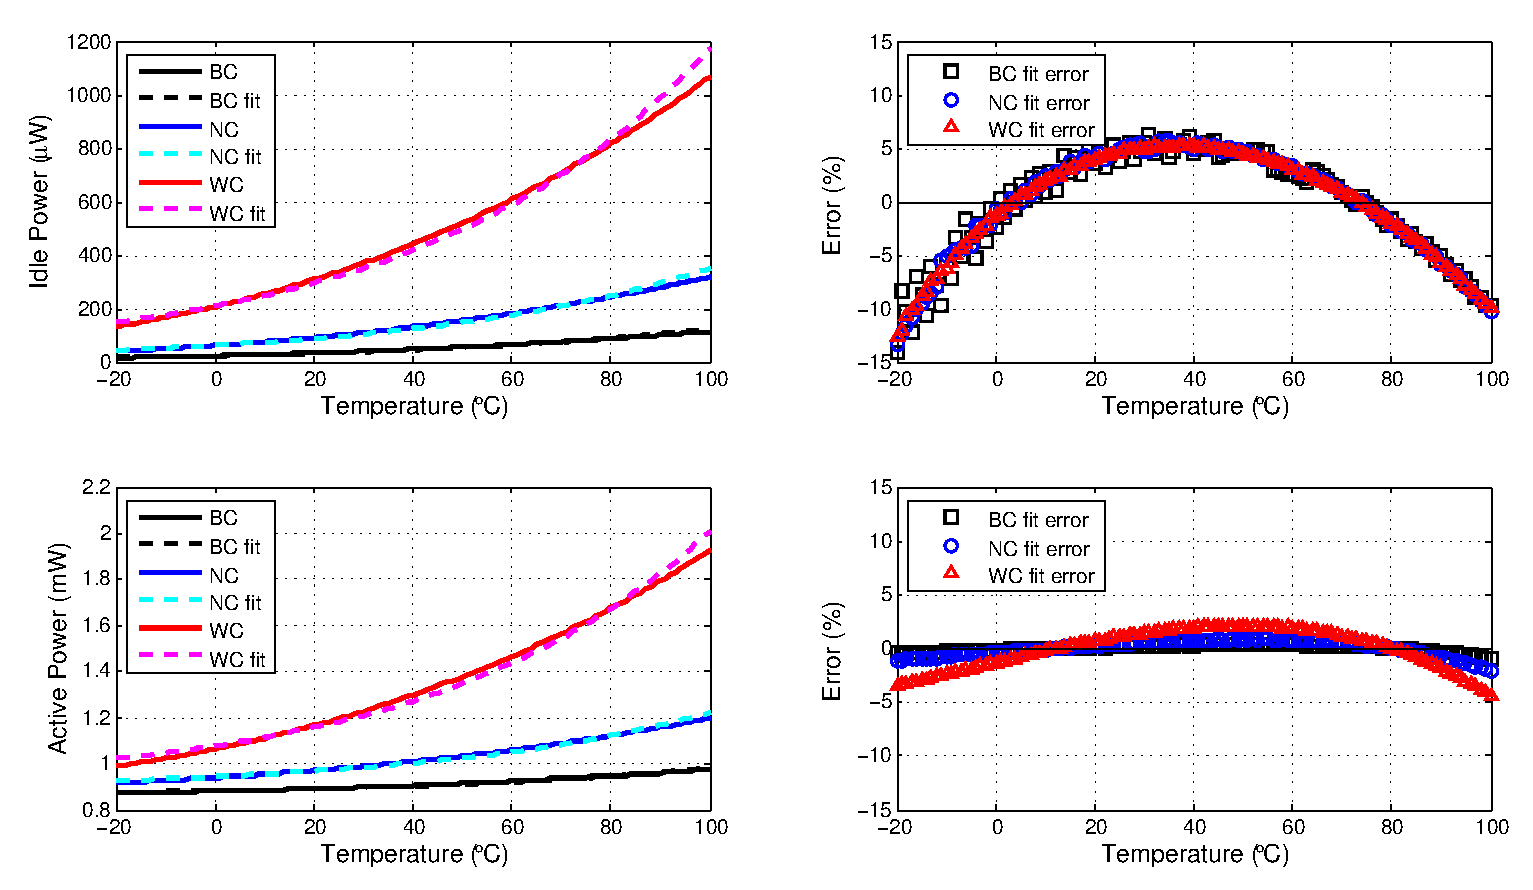
\includegraphics[width=0.47\textwidth, clip=true, trim=5in 0in 0in 2.855in]{figures/powerlearning}}\\ \vspace{0mm}
\caption{\label{fig:powerlearning}Modeling sleep and active power through linearization. }
\end{figure*}

\subsection{Online Modeling of Sleep and Active Power}
As discussed in Section \ref{sec:variability}, both sleep power and active power are nonlinear functions of temperature.  The vast majority of this nonlinearity comes from leakage and sub-threshold currents which dominate in $P_s$. In general, modeling these nonlinear curves could prove difficult with limited resources and without, in many cases, fully fledged math libraries. For example, nonlinear regression is often performed as an optimization problem using a specialized library such as NLopt, requiring more than 300 kB of program space in order to do even rudimentary optimization routines \cite{nlopt} and prohibiting its use in many low power platforms.   Fortunately, the models in Section \ref{sec:variability} describing $P_s$ result in a function that is very closely exponential.  Knowledge of the shape of this function allows us to linearize the model which in turn allows the use of linear regression to accurately model $P_s$.  Specifically, linear regression is run on $\log(P_s)$, giving offset $b_s$ and slope $m_s$.  The desired sleep power model is likewise computed as $P_s(T) \approx \exp(b_s + m_sT)$. After $P_s(T)$ has been computed, $P_a(T)$ can be modeled by subtracting $P_s(T)$ from active power measurements and continuing with a second linear fit.  

The error between the models described in Section \ref{sec:variability} and the linear approximation methods described above is shown in Figure \ref{fig:powerlearning} for three separate power instances representing the best-case (BC), nominal-case (NC), and worst-case (WC) for a 45nm Cortex M3 processor---(a) shows the sleep power model with the corresponding error in (b), and (c) shows the active power model with the corresponding error in (d).  For the linear approximation of $P_s$ on the temperature range [-20$^\circ$C, 100$^\circ$C], the worst case error is around -15\% while on a more temperate range of [0$^\circ$C, 80$^\circ$C] the worst case error is around 5\%.  For most temperature profiles this accuracy will be adequate, but deployments in extreme environments can experience the detriments of errors in the linear model of $P_s$.  Because of the added baseline in $P_a$, the corresponding prediction error is drastically reduced---less than 2\% across [-20$^\circ$C, 100$^\circ$C] for the best-case and nominal instances and less than 5\% for worst-case.  These errors can be further reduced using nonlinear regression methods if the computational resources are not a limiting factor; for VaRTOS we have chosen a lightweight design so that resource-constrained low power processors---those that are likely to be used in long lifetime sensing tasks---can easily perform the necessary computations. 

Models for both $P_s$ and $P_a$ take some time to converge, before which an accurate prediction for the optimal duty cycle $d_{sys}^*$ cannot be calculated. Convergence is aided by variations in temperature, giving a variety of points on the $T\rightarrow\{P_s, P_a\}$ curves, and hurt by noise variance in power sensors.  For example, if our sensor for $P_s$ takes hourly measurements with additive white Gaussian noise $\sim\normal(0, ~5\mu\text{W})$, the percentage error of our model has reached a reasonable accuracy after 40 hours and is nearly fully converged after 60 hours.  This is shown in Figure \ref{fig:powerconvergence} for 190 different locations within the United States with between 1 and 9 years of hourly data in all locations and for processor instances with best-case, nominal-case, and worst-case power consumption. For the results that follow, both sleep and power models will be fit after 40 points (40 hours) of data have been collected.  


\begin{figure*}[t]
\centering
{\centering
\begin{minipage}{0.47\textwidth}
  \centering
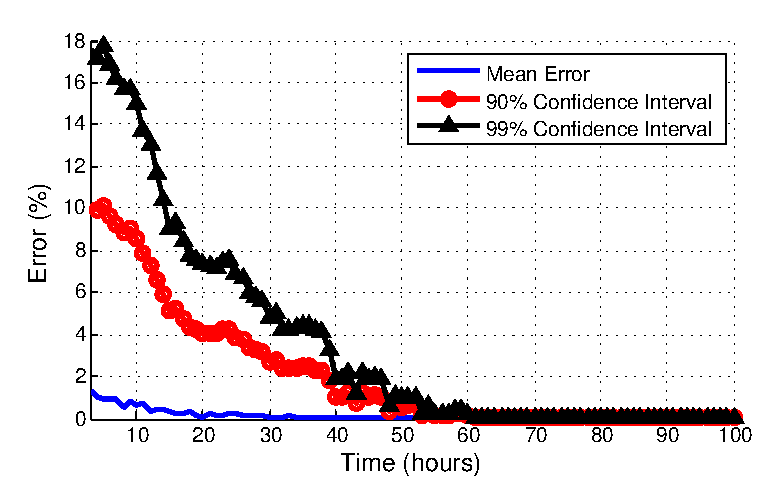
\includegraphics[width=\textwidth]{figures/powerconvergence}
  \captionof{figure}{\label{fig:powerconvergence}Error convergence for sleep power modeling. Shown are the mean errors, 90\% confidence, and 99\% confidence intervals for errors vs. the steady state models. }
\end{minipage}
\hspace{.04\textwidth}
\begin{minipage}{0.47\textwidth}
  \centering
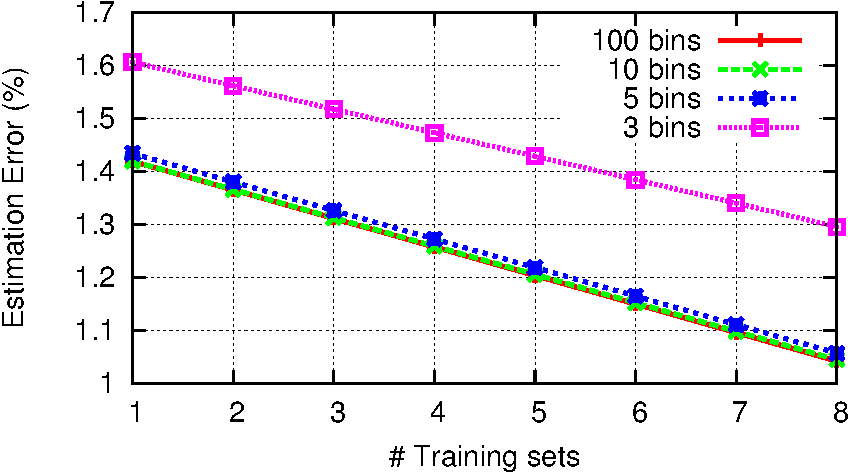
\includegraphics[width=\textwidth]{figures/temperature_estimation_error}
  \captionof{figure}{\label{fig:tempestimation}Error in average power estimation for temperature models constructed from varying numbers of training years ($x$-axis) and with a set number of histogram bins. }
\end{minipage}
}
\end{figure*}

\subsection{Online Modeling of Task Computation}
\label{sec:vartos:knobtime}
Active time per task $t_{a,i}$ can be measured in a number of ways (for example, using hardware timer snapshots at the context swap level).  Given a method for measuring $t_{a,i}$, $\mathcal{K}_i$ is arrived at by systematic perturbation of $k_i$ within the range $[k_{i,min}, k_{i,max}]$. Specifically, $k_i$ is repeatedly increased by $\Delta = {k_{i,max} - k_{i,min} \over n}$ where $n$ is the number of points in the regression, kept sufficiently low ($n = 4$ in our case) to minimize memory footprint.  Between each perturbation in $k_i$, the task is allowed to run for a time period sufficiently long enough to capture active time measurements for tasks with very infrequent activity.  In the applications presented here, this supervisory period is set at $t_{super} = 1$ hour, meaning the mappings $\mathcal{K}_i$ are calculated after 4 hours. Task duty cycles are calculated as $d_i = (\sum t_{a,i})/t_{super}$. Note that $\mathcal{K}_i$ is a linear transformation from $k_i$ to $d_i$ and thus $k_i$ should translate linearly into active time for that task.  In Section \ref{sec:casestudies} we explore the effects of violating this assumption. 

Many tasks are likely to make heavy use of interrupt subroutines (e.g. for analog to digital conversion, radio transmission, serial communication, etc.).  In order for this time to be accounted during the supervisory period, we provide functionality for assigning each subroutine to a particular task using a handle provided during task creation.  For example, on entering a subroutine the \inlinecode{taskEnterISR( taskHandle)} command is invoked with a matching \inlinecode{taskExitISR} upon finishing the subroutine. Again, as mentioned in Section \ref{sec:optimization:maxutil}, in some cases additional peripheral power will be expended during these subroutines.  The metric $t_{a,i}$ reflects only processor power expenditure, and thus peripheral power usage must be modeled separately by modifying $\mathcal{L}_i$. 

\subsection{Controlling Task Active Time}
\label{sec:vartos:tasktime}
In the same way that $k_i$ is perturbed to model $\mathcal{K}_i$ in the previous section, $k_i$ is also commanded by the operating system to achieve $d_i^*$ as calculated by Algorithm \ref{alg}. Knob control is passed from user to operating system at task creation, making the full task creation call using the modified FreeRTOS kernel:

\begin{verbatim}
xTaskCreate( TaskFunction, "name", StackSize, Priority, &TaskHandle,
                                        &TaskKnob, k_min, k_max, p_i);
\end{verbatim}

By its nature, \inlinecode{TaskKnob} serves as a discrete representation of $k_i$ and therefore introduces quantization errors into the optimization routine.  In particular, the smaller the difference between $k_{i,min}$ and $k_{i,max}$, the coarser the granularity of \inlinecode{TaskKnob} becomes and therefore the poorer the achievable resolution of $d_i$ becomes.  As an extreme example, if $k_{i,min} = 1$ and $k_{i,max} = 2$, then \inlinecode{TaskKnob} can only take on 1 of 2 values and thus 1 of 2 $d_i$ values, perhaps far away from $d_i^*$. Similarly, even if \inlinecode{TaskKnob} is constructed in such a way that it has fine granularity, $d_i^*$ might not be within the range $[\mathcal{K}_i[k_{i,min}],~\mathcal{K}_i[k_{i,max}]]$. When $d_i^*$ is less than $\mathcal{K}_i[k_{i,min}]$, task $\tau_i$ consumes more energy than it is allotted and the system is likely to die prematurely.  If $d_i^*$ is greater than $\mathcal{K}_i[k_{i,max}]$, however, it may simply mean that even though additional energy can be allotted to task $\tau_i$, no additional utility would be gained and so achieving a lifetime greater than $L$ is acceptable. 

\subsection{Temperature Models}

Equations \ref{eq:linprog_fin} and \ref{eq:dstar} require that we know the temperature distribution $\pmb{f}_T$ in order to calculate $d_{sys}^*$ and the individual task ratios $\{d_1^*,\ldots,d_N^*\}$. We performed several simulations with results indicating that learning $\pmb{f}_T$ online is infeasible, as it takes the entirety of a year to develop an accurate histogram of the temperature values seen at a given location.  Fortunately, similar simulations show that a very coarse representation of the temperature profile suffices for accurate calculations of $d_{sys}^*$, and furthermore temperature profiles change very little from year to year for a given location. Figure \ref{fig:tempestimation} shows how certain temperature models affect the error in predicting average power consumption for $P_s$ across the lifetime of the system (in this case, 1 year).  The $x$-axis here represents the number of years of temperature data used to train the model before testing on a single year.  Each line represents a certain number of bins used in a histogram representing $\pmb{f}_T$ for a given location. This figure makes two noteworthy points: first, the decreasing estimation error indicates that temperature profiles change very little from year to year, and because of this using multiple years to build $\pmb{f}_T$ only serves to decrease the prediction error in years to come; second, while a 3-bin histogram is inadequate to fully represent the temperature profile for a given location, there is very little benefit in representing $\pmb{f}_T$ with more bins than 5 and even less so with more than 10.  Because of this, for a given location we train with as many previous years as are available and we use a 10-bin histogram to represent $\pmb{f}_T$.  
%Additionally, high resolution is not required on the frequencies of each of these bins, so a single byte per bin suffices, giving a 10 byte representation of the entire temperature profile. This 10 byte histogram is generated \emph{a priori} given a desired deployment location. 


\subsection{User Programming Model}
\label{sec:vartos:tool}
Much of the effort in creating VaRTOS is in making the process transparent to the developer and easing the burden of accounting for variable task power consumption.  In addition to the challenges that come with embedded programming in general, developers need only provide the following information:
(1) Energy budget $E$ measured in Joules;
(2) Lifetime goal $L$ measured in hours;
(3) Deployment location if it belongs in the VaRTOS database or corresponding coarse $\pmb{f}_T$ if not;
(4) $k_{i,min}$, $k_{i,max}$, and priority scaling factors $p_i$;

%Information in (4) above is provided as shown in Section \ref{sec:vartos:tasktime}.  The remaining information is specified as part of a structure that is handed off to the OS scheduling subroutines upon initialization.  
Information required from the developer is therefore very minimal, though in many circumstances it is not readily apparent how different user inputs---particularly for knob values and priorities---will affect the operation of the system.  In order to provide more intuition regarding the various parameters the developer is tasked with supplying, we have developed a simple tool in MATLAB as shown in Figure \ref{fig:gui}.  This tool allows the developer to specify an energy budget and lifetime goal to guide the optimization process.  Developers further specify clock frequency, instance type, a certain geographical location, and the various tasks to be scheduled.  Perhaps the most difficult part of this tool is in estimating how many cycles each task will take per knob value. This tool only gives a rough estimate of how the true deployment will behave, but it helps guide the developer's choices along the way.  

\begin{figure}
\centering
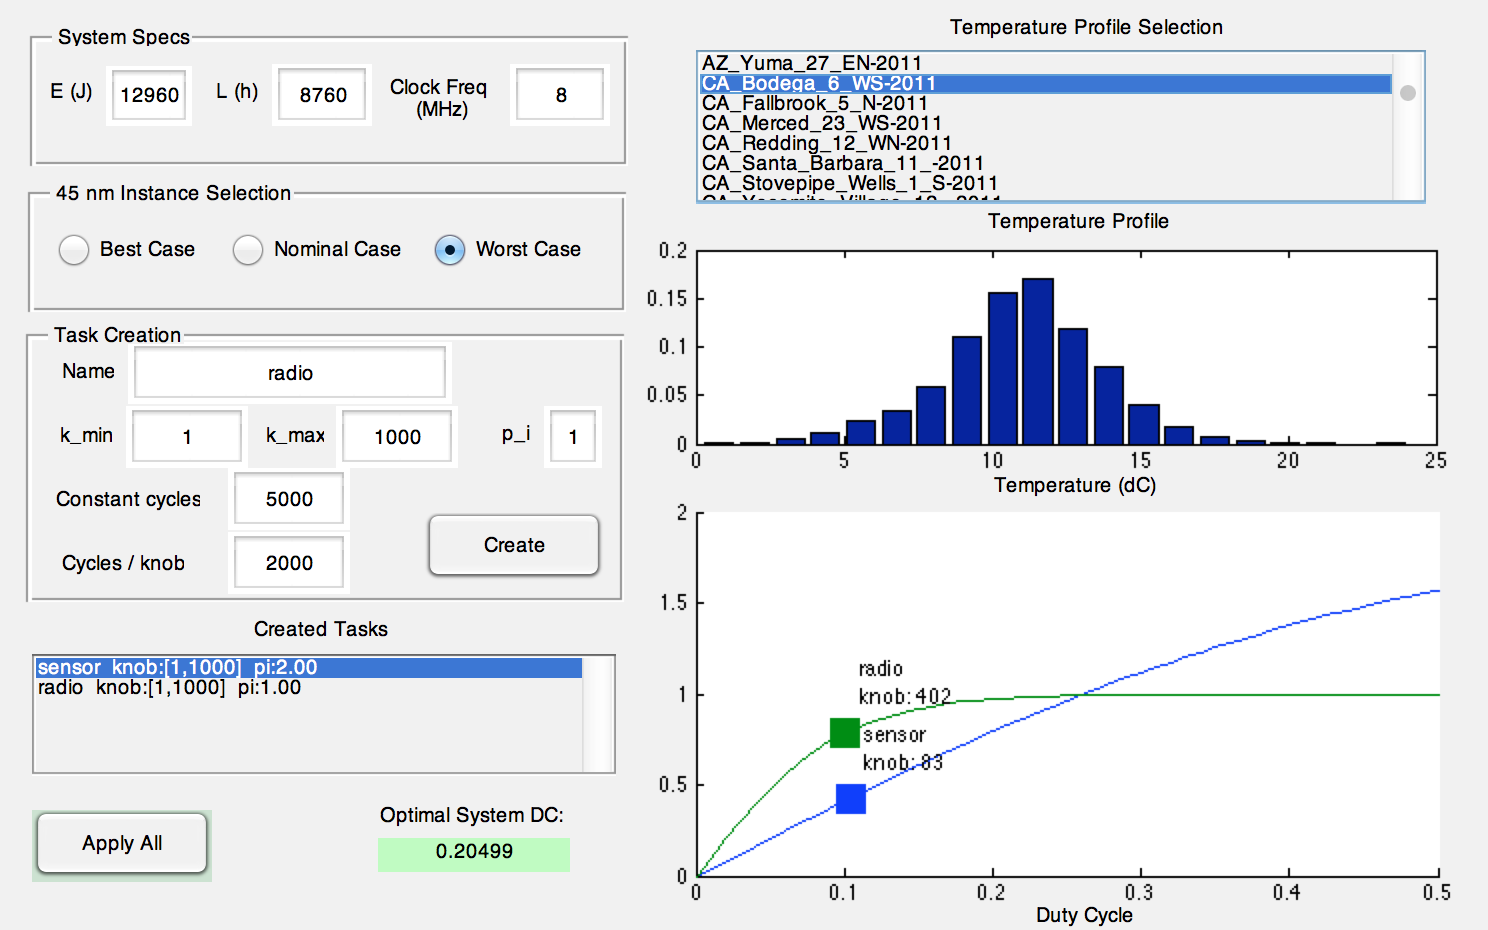
\includegraphics[width=1\textwidth]{figures/matlab_gui}
\caption{\label{fig:gui}A tool for guiding developers using VaRTOS. Users input various system specifications along with task prototypes and a geographical location, and the corresponding optimal duty cycle $d_{sys}^*$ and knobs $k_i^*$ are displayed. }
\end{figure}

\subsection{Operation}
\label{sec:vartos:operation}

\begin{figure}
\centering
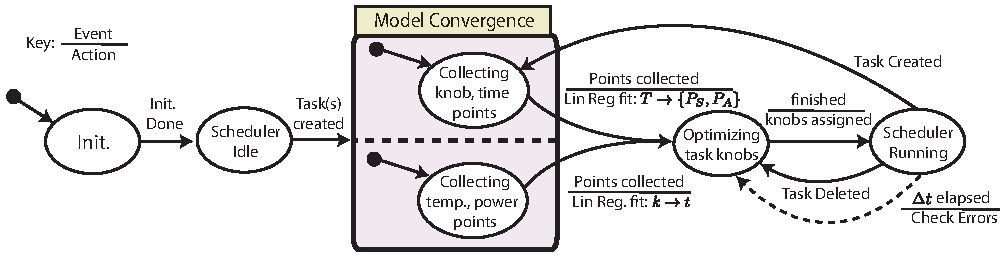
\includegraphics[width=1.0\textwidth]{figures/statechart.pdf}
\caption{\label{fig:statechart}VaRTOS state chart, showing model convergence and optimization states.}
\end{figure}

In this section we discuss the operation of VaRTOS from a broader perspective, using the state chart depicted in Figure \ref{fig:statechart}. To begin, the system is initialized with task creations, energy and lifetime specifications, and a location-specific temperature model.  If at least one task has been created, the scheduler begins operation and we enter a model convergence state.  While in this state, hourly temperature and power measurements are collected and knob values are incremented every $t_{super}$ seconds (see Section \ref{sec:vartos:knobtime}) to construct $\mathcal{K}_i$. The optimization routine cannot complete until both models have converged, after which linear regression and linearization are used to fit the knob to duty cycle and temperature to power curves, respectively. This brings us to the optimization state.  Here the various $d_i^*$ are calculated as per Algorithm \ref{alg}, and the corresponding knob values (calculated by inverting $\mathcal{K}_i$) are assigned to the appropriate tasks. At this point we begin steady state operation in the `Scheduler Running' state. Potential reasons for leaving this state include task creation (necessitating learning the new task's $\mathcal{K}_i$ and re-optimizing) or task deletion (requiring only re-optimization). Because the modeling tasks only run on an as-needed basis, these are implemented as OS tasks with null-valued knobs.  This allows for easy suspension and resumption of these tasks as necessary. 

The dashed line on Figure \ref{fig:statechart} represents an optional feedback error-checking mechanism that can help for online readjustment of poor initial power model construction (e.g. for cases where measurement of $P_s$ and $P_a$ is particularly noisy).  This can be done by comparing true energy expenditure with predicted expenditure, if such a sensor exists, and using the error to apply proportional feedback, though we present no results regarding this extension in this paper. 




%\begin{figure}
%\centering
%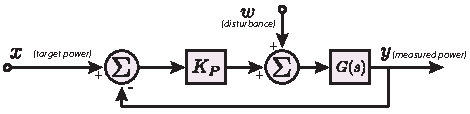
\includegraphics[width=0.5\textwidth]{figures/controlloop.pdf}
%\caption{\label{fig:state chart}state chart}
%\end{figure}




 % Paul
\section{Experimental Setup}
\label{sec:methods}

We implemented VaRTOS as a series of architecture-independent extensions to FreeRTOS~\cite{freertos}, a popular open-source real-time operating system. FreeRTOS provides typical operating system abstractions such as preemptive scheduling of multiple tasks, synchronization primitives, and dynamic memory allocation with low overhead and small memory footprint. For our evaluation, we use the TI Stellaris LM3S6965 port of FreeRTOS. The LM3S6965 is a microcontroller based on an ARM Cortex-M3 core, and is representative of the low-power platforms targeted by VaRTOS.

VaRTOS relies on a temperature and instance-dependent power model to perform its optimizations and requires appropriate sensors from its underlying hardware platform to build this model. Temperature sensors are typically embedded into most sensing platforms. Energy consumption and power in various processor modes may be measured directly (e.g. as in~\cite{leap}), or indirectly estimated from remaining battery capacity (e.g. with a ``smart'' battery or as in~\cite{Lachenmann}). Low-cost probes for variability vectors (including aging, frequency, and leakage power) may be embedded into processor cores, and exposed to software as digital counters~\cite{Chan:2012}. 

We evaluate VaRTOS with a series of case study applications under different hardware instances and deployment scenarios (temperature profiles) across a lifetime of 1 year. Because it would be impractical to physically deploy these applications, we rely on VarEMU~\cite{varemu}, a variability-aware virtual machine monitor.

VarEMU is an extension to the QEMU virtual machine monitor~\cite{qemu} that serves as a framework for the evaluation of variability-aware software techniques. VarEMU provides users with the means to emulate variations in power consumption in order to sense and adapt to these variations in software. In VarEMU, timing and cycle count information is extracted from the code being emulated. This information is fed into a variability model, which takes configurable parameters to determine energy consumption in the virtual machine. Through the use (and dynamic change) of parameters in the power model, users can create virtual machines that feature both static and dynamic variations in power consumption. A software stack for VarEMU provides virtual energy monitors to the operating system and processes. With the exception of the driver that interfaces with the VarEMU energy counters, VaRTOS running in VarEMU is unmodified from its version that runs on physical hardware.  

When starting VarEMU, we provide a configuration file with parameters for the power model described in Section~\ref{sec:variability}. For most test cases, we evaluate the system with three instances (nominal, best-case, and worst-case) as shown in Figure~\ref{fig:power}. When necessary for the evaluation, further instances are generated according to SPICE simulation results as described in~\ref{sec:variability}. We also provide a trace of temperature based on hourly temperature data from the National Climactic Data Center~\cite{ncdc} for three locations: Mauna Loa, HI (`best-case': mild temperature, very little variation), Sioux Falls, SD (`nominal-case': average temperature and variation), and Death Valley, CA (`worst-case': extreme temperature and variation). For every hour elapsed on the Virtual Machine, VarEMU reads a new line from the temperature trace file and changes the temperature parameter in the power model accordingly. In order to accelerate the simulation (which would otherwise run in real-time), we use a time scale of 1:3600, resulting in a total simulation time of approximately 2.5 hours for a lifetime of one year.




 % Lucas
\section{Evaluation}
\label{sec:evaluation}
In this section we present results regarding the ability of VaRTOS to maximize utility by modification of task knob values as well as the corresponding error in energy consumption vs. the specified energy budget.  Finally, we evaluate the VaRTOS architecture in terms of both energy and memory overheads.  

\subsection{Minimizing Energy Consumption Error}

\begin{figure*}
\centering
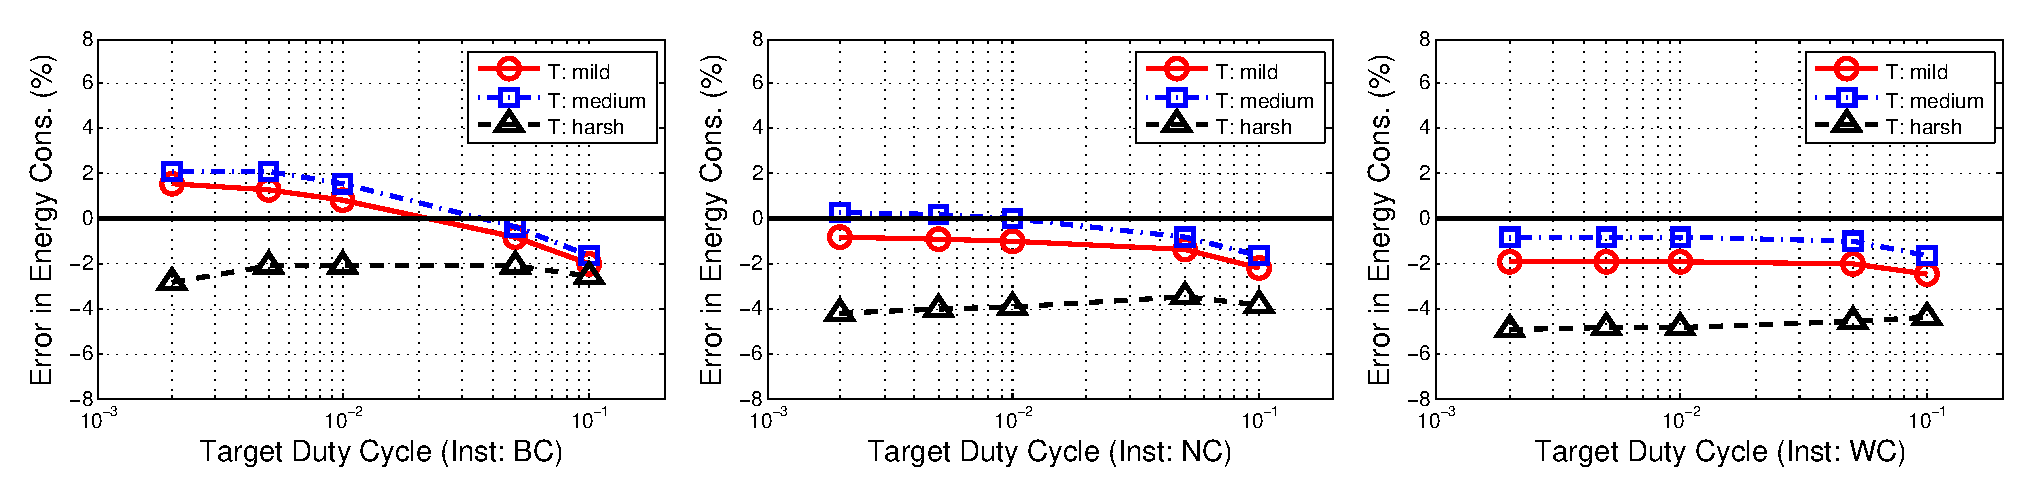
\includegraphics[width=1\textwidth]{figures/app1_nonoise}
\caption{\label{fig:app1_dc}Error in energy consumption for various optimal duty cycles and for mild, medium, and harsh environments.  From left to right, figures represent the best case, nominal case, and worst case power instances in 45 nm.}
\end{figure*}

%\begin{figure*}
%\centering
%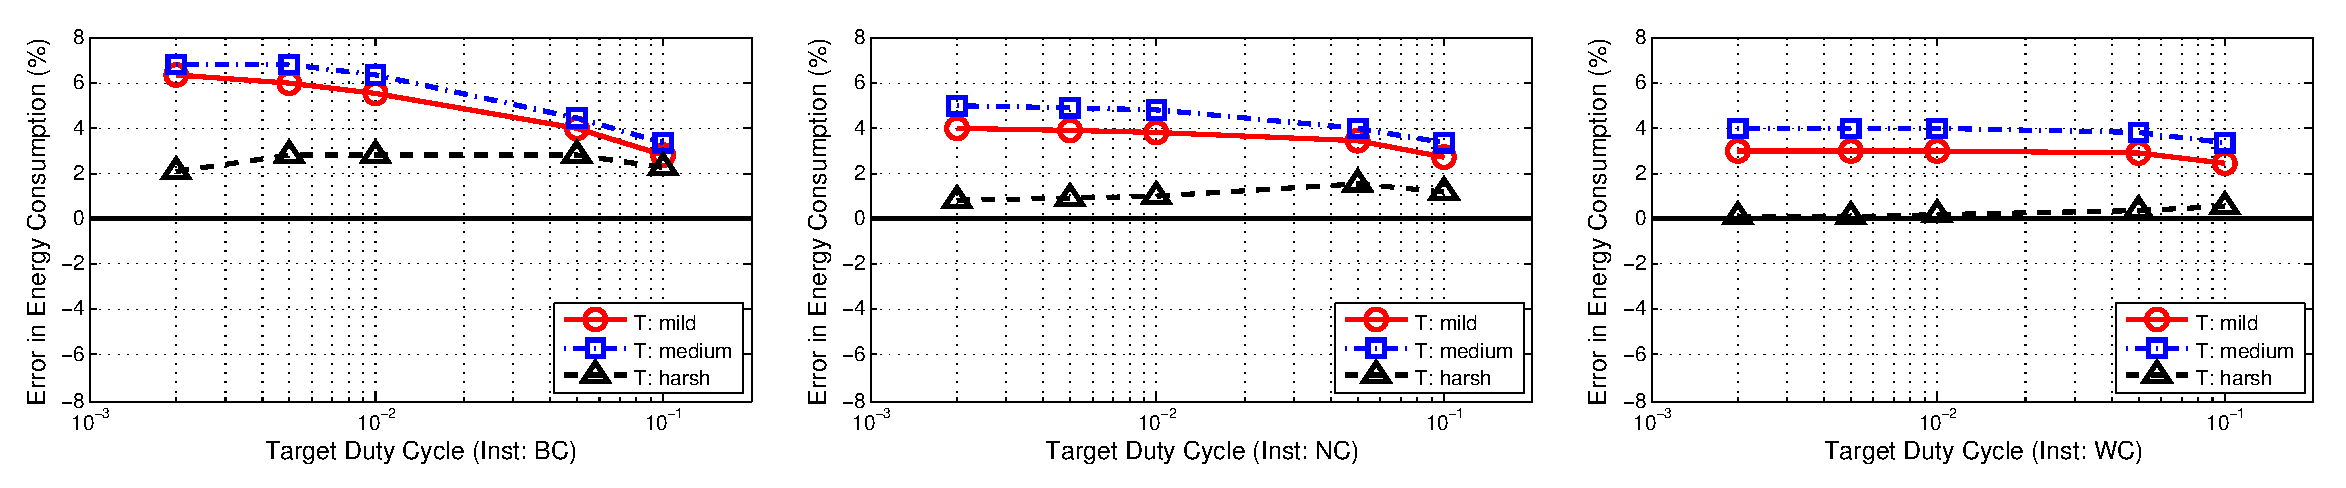
\includegraphics[width=1\textwidth]{figures/app1_guardband.eps}
%\caption{\label{fig:app1_dc_guardband}App 1 results, no noise}
%\end{figure*}

In order to achieve accurate energy consumption to meet a lifetime goal, VaRTOS needs to accurately be able to achieve the overall system duty cycle $d_{sys}^*$.  To test this, we constructed a simple application with only a single task containing a knob with fine granularity values.  Then, using the tool shown in Figure \ref{fig:gui}, we specified various values for $E$ and $L$ that would ideally lead to a particular $d_{sys}^*$ for each of the power instance models (best-, nominal-, and worst-case) as well as three temperature profile instances (harsh, medium, and mild).  The target duty cycles were $d_{sys}^* \in \{0.002, 0.005, 0.01, 0.05, 0.1\}$, or from 0.2\% up to 10\%, and the resulting errors in energy consumption are shown in Figure \ref{fig:app1_dc}.  Note that errors are larger in harsher environments, where any errors in the power models will be magnified.  In the worst case, an error of 4.9\% in energy consumption is seen for a harsh environment and for the worst-case power instance (far right plot in Figure \ref{fig:app1_dc}). This means that, in the worst case, a 5\% guard band in lifetime or in energy is necessary if the lifetime goal is to be treated as a hard constraint. 

To give more intuition into what this error in energy consumption means, we compared energy consumption for tasks running in VaRTOS (modeling power on a per-instance basis) with those assuming `worst-case' power consumption.  True worst-case power consumption is difficult to define, due to the long tail distribution for power across temperature.  Because of this, we define worst-case power as the average power consumption for the worst-case instance from Section \ref{sec:methods} across the temperature range $[0^\circ C,~45^\circ C]$, particularly $P_s = 330 ~\mu$W and $P_a = 1.187$ mW.  Figure \ref{fig:app1_energy} shows the disparity between the two.  Without per-instance power modeling, energy consumption is in some cases over 70\% off, and in only one case is it below 10\% error.  With per-instance power modeling using VaRTOS, the error has dropped to below 2\% in most cases and around 5\% in the worst case. Note that a positive percent error means a surplus in energy after the lifetime has been met while a negative means an energy deficit (and likewise a premature death).  Energy errors are mostly positive here because of the worst-case power assumption. 

Similarly, Figure \ref{fig:app1_dc2} shows the cause of this energy error disparity---the duty cycle ratio remains constant if worst-case power is assumed while it is allowed to vary when instance-specific power modeling is introduced.  This will translate into an increase in the quality of service for a particular application (e.g. more data collected, a higher communication rate) by using what would have been surplus energy. 

\begin{figure*}[t]
\centering
{\centering
\begin{minipage}{0.47\textwidth}
  \centering
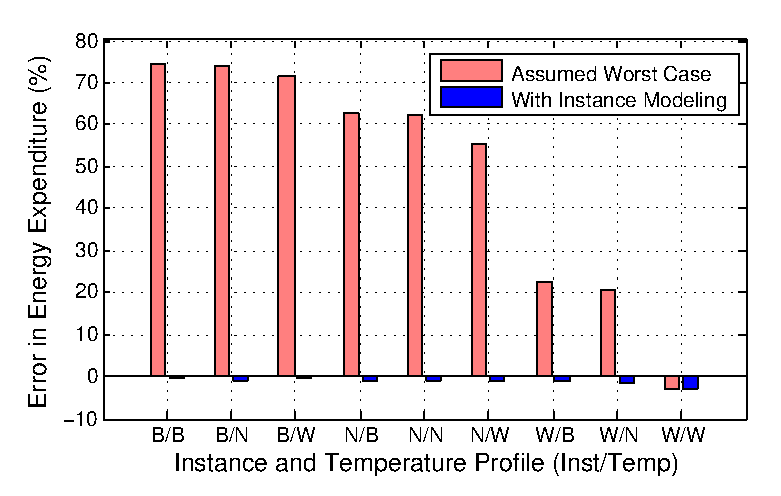
\includegraphics[width=\textwidth]{figures/app1_energycomp}
  \captionof{figure}{\label{fig:app1_energy}Errors in energy consumption for a single-task application for worst-case power assumptions and per-instance power modeling.}
\end{minipage}
\hspace{.04\textwidth}
\begin{minipage}{0.47\textwidth}
  \centering
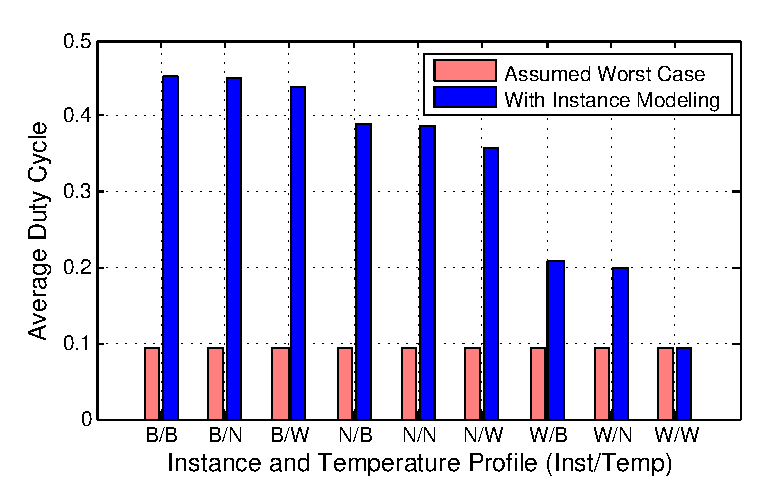
\includegraphics[width=\textwidth]{figures/app1_dutycycles}
  \captionof{figure}{\label{fig:app1_dc2}Average duty cycles of a single-task application for worst-case power assumptions and per-instance power modeling. }
\end{minipage}
}
\end{figure*}



\begin{figure}
\centering
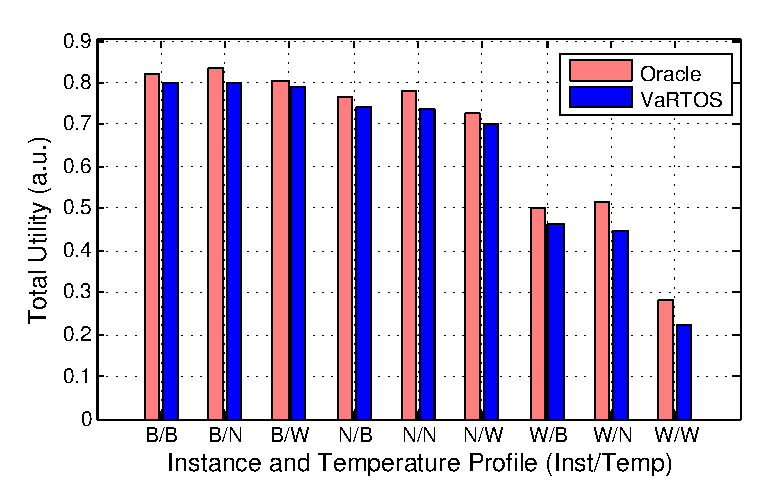
\includegraphics[width=0.47\textwidth]{figures/app1_oracle}
\caption{\label{fig:app1_oracle}Total utility, $u_{sys}$, for VaRTOS vs. the oracle system.}
\end{figure}

\subsection{Utility and Oracle Comparison}
The results in the previous section showed that VaRTOS is able to meet a given energy budget with low error, resulting in an accurate system lifetime.  In Section \ref{sec:optimization} we argued that spending would-be surplus energy will increase system utility.  In this section, we substantiate this claim by comparing the utility of the single task app running in VaRTOS to that of an all-knowledgeable oracle system.  Unlike the true VaRTOS system, the oracle system is allowed the following privileges: (1) complete knowledge of the temperature profile for the test year; (2) perfect knowledge of task behavior (i.e. $\mathcal{K}_i$); (3) full accuracy models for $P_s$ and $P_a$; and (4) zero overhead for optimization routines.  Figure \ref{fig:app1_oracle} shows the utilities for both the oracle and VaRTOS.  In most cases VaRTOS achieves within 10\% of the oracle utility, and is as much as 20\% off in the worst case.  Note that this comparison is specific to the construction of utility $u_i$ as defined in Equation \ref{eq:util}, and other utility curves may cause variations in this metric.


\subsection{Energy and Memory Overhead}
Energy consumption by the various VaRTOS subsystems must be minimized in order to prevent worsening the very thing we are trying to correct.  Similarly, the memory required for VaRTOS must be kept reasonably low in order to make it a viable option for resource-constrained platforms.  \\

\noindent\emph{\underline{Memory Overhead:}}
The amount of program memory (.text, .data) and volatile memory required for VaRTOS depends on the application that the developer is designing.  As a baseline, VaRTOS requires a modest increase in the `.text' section over the vanilla FreeRTOS framework from 2.29 kB to 6.80 kB ( a 4.51 kB increase).  This includes a lightweight library for math functions required for optimization routines (including exponential, logarithmic, and square root functions) as well as a preemptive scheduler.  If a full math library needs to be used for the application itself, these functions can be replaced and the overhead amortized.  In terms of volatile memory, an additional 508 bytes baseline is required (480  bytes of this is due to the power learning procedure and, if the developer is so motivated, can be reused after the models have converged).  An additional 46 bytes per task is also required for knob modeling and other parameters.  Finally, the temperature profile is stored in program ROM as a constant array and consumes only 10 additional bytes. \\

%
%memory: 40 floats for Ps, Pa, temp: 120 floats for power convergence, can be freed if memory management available. float for (psslope, psoffset, paslope, paoffset, optimaldc). int for (lifetime, energy). 
%
%added memory per task: int for knob, kmin, kmax, float for pi, float for time model times (4), float for Koffset and Kslope and dcopt. also (4) for knobs in the array 
%

\noindent\emph{\underline{Energy Overhead:}}
The largest energy overhead in VaRTOS comes from the scheduler itself, which, if context swaps occur every 10 ms, causes a baseline system duty cycle of 0.1\%. This ratio can be decreased if coarser granularity context swaps are acceptable.  The power consumption attributed to this 0.1\% depends on the power consumption of the processor and the environmental temperature, but in the worst case it consumes $P_{os} = 0.001\cdot(1.187~mW) + 0.999\cdot(330~\mu W) = 331~\mu W \approx P_s$. In other words, the sheduler adds only marginal power consumption on top of the baseline sleep power. 

Other potential energy consuming processes attributed to VaRTOS include knob modeling, power measurement and fitting, finding the optimal $d_{sys}^*$, and finding the optimal knob values.  The amount of processing time spent in these tasks is negligible:  reading power and temperature takes 250 $\mu$s and occurs only 40 times over the course of a deployment (10 ms total); knob perturbations take 48 $\mu$ s and occur 4$\cdot N$ times (for $N$ tasks); performing a 40-point linear regression (for power curves and as an upper bound for modeling $\mathcal{K}_i$) takes 40 ms and occurs twice ($P_s$ and $P_a$) per deployment and once per task; finding $d_{sys}^*$ takes 54 ms and occurs once unless tasks are deleted and created after the initial optimization; and finally finding optimal $d_i^*$ and $k_i^*$ values takes 345 $\mu$s.  In total, these added tasks consume less than 1 mJ in the worst-case for a 1 year deployment, a negligible overhead if our energy budget is 12960 Joules (2 AAA batteries) as in the following section. Note, however, that (1) taking power and temperature measurements is likely to consume additional power for analog to digital conversions and (2) a more difficult calculation in energy overhead comes from the result of perturbing knob values in the modeling phase for $\mathcal{K}_i$.  The latter depends on the nature and number of tasks, as well as the length of $t_{super}$. 



















 % Paul
\section{Case Studies}
\label{sec:casestudies}

We have shown in Section \ref{sec:evaluation} that VaRTOS can accurately achieve a desired lifetime goal given an energy budget, and we made the claim that using would-be surplus energy will increase application performance.  Here we provide several simulated case studies to substantiate this claim, using the same experimental setup described in Section \ref{sec:methods} with additional virtual peripherals as needed. For these case studies, the energy budget is set at a constant 12960 Joules, corresponding roughly to that of 2 AAA batteries in parallel.  In addition, the lifetime goal is set at 8760 hours, or 1 year. 

\subsection{Multi-Agent Applications}
\label{sec:casestudies:localization}

\begin{figure}
\centering
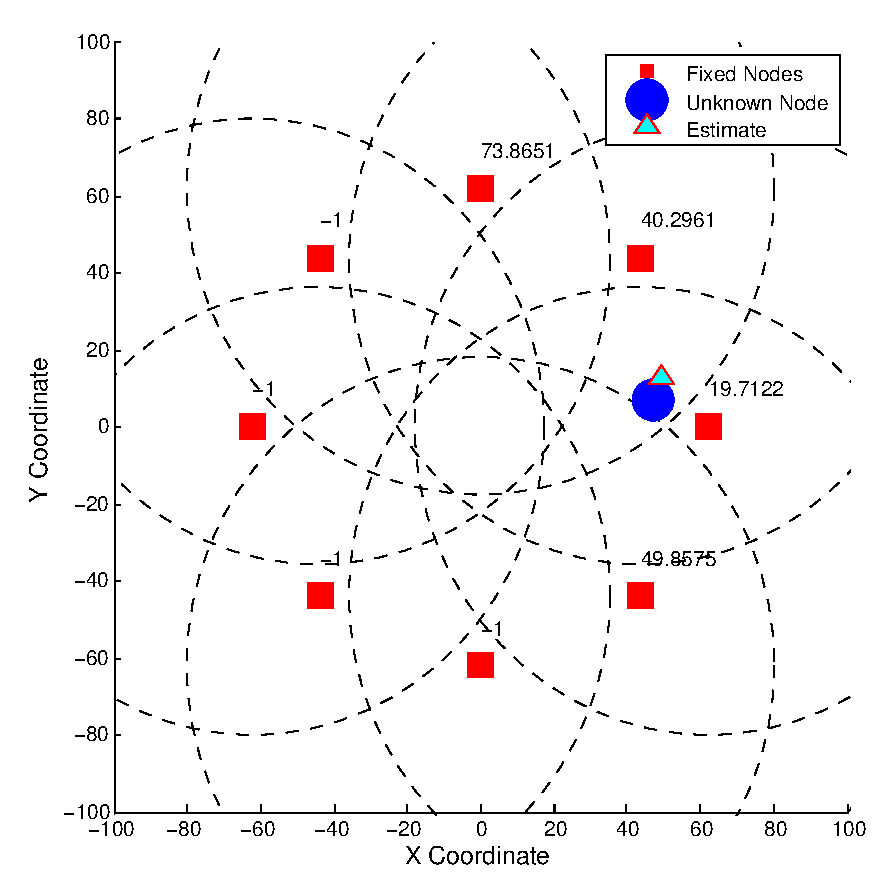
\includegraphics[width=0.5\textwidth]{figures/localization_snapshot2}
\caption{\label{fig:loc_overview}Multi-agent localization application: the square nodes with known location attempt to localize the unknown circle node through consensus. }
\end{figure}


Oftentimes a system is composed of multiple nodes connected by either wired or wireless communication.  As an example, consider a network of 8 nodes with wireless radio capabilities.  Each node is capable of sensing a noisy measurement that corresponds roughly to the distance of some unknown object to the node, whose location is known.  For example, these nodes could be taking audio measurements and inferring the distance of a vehicle traveling around a track.  From these distance measurements, we would like to estimate the $(x,y)$ coordinate of the unknown vehicle.  This system is illustrated in Figure \ref{fig:loc_overview}, where the unknown object makes a counter-clockwise path and the known sensor nodes take noisy measurements if the object is within their radius of observation, shown with dashed circles.  Here the unknown object is traveling on a track of 300 m circumference at the speed of 0.4 km/h. The 8 known nodes can `observe' a linear distance to the unknown node if it is within 80 m.  Each node operates two tasks: (1) a radio with a variable frequency transmission, and (2) a sensor that samples a variable number of points and averages the samples.   Allowing the radio more active time will reduce the latency in reported estimates of the unknown node, while allowing the sensing task more time will generate more reliable estimates.  The task priorities $p_i$ along with the tool described in Section \ref{sec:vartos:tool} would help a developer give preference to one or the other. For the sake of our comparison, we keep the priorities the same and choose knob ranges to allow the sensor to average between 1 and 100 samples and to allow the radio to transmit anywhere from 10 Hz to 0.1 Hz.  Because these peripherals are simulated, each task has been padded with NOP instructions in order to simulate work that an actual system might be doing.  If we look at a 1000 minute time slice of the estimation process as shown in Figures \ref{fig:loc_error_var} and \ref{fig:loc_error_novar}, we see that the variance of the estimation error is much greater if we assume worst-case power and thus average fewer samples and much less if we use VaRTOS with instance-specific power models.  When many samples are averaged, the noise is reduced and each estimate is the result of consensus between more reliable measurements.  In other words, for the same lifetime specifications, the system using VaRTOS greatly outperforms the system that assumes worst-case power consumption.  While the deployment assuming worst-case consumption suffers from an average error variance of 59.7, the VaRTOS deployment has an average error variance of only 26.9, a 54.9\% improvement.  The periodic nature of the high variance peaks in estimation error for both Figures \ref{fig:loc_error_var} and \ref{fig:loc_error_novar} can be attributed to the circular nature of the application setup (Figure \ref{fig:loc_overview}).  When the unknown object comes within view of nodes with less reliable measurements, the estimation error is much poorer. 

\begin{figure*}[t]
\centering
{\centering
\begin{minipage}{0.47\textwidth}
  \centering
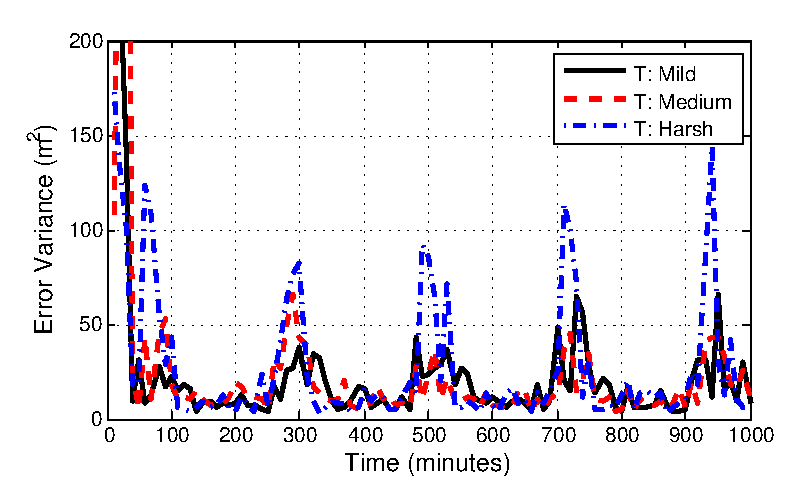
\includegraphics[width=\textwidth]{figures/localization_variance_var}
  \captionof{figure}{\label{fig:loc_error_var}Reduced error variance for multi-agent localization using instance power modeling with VaRTOS}
\end{minipage}
\hspace{.04\textwidth}
\begin{minipage}{0.47\textwidth}
  \centering
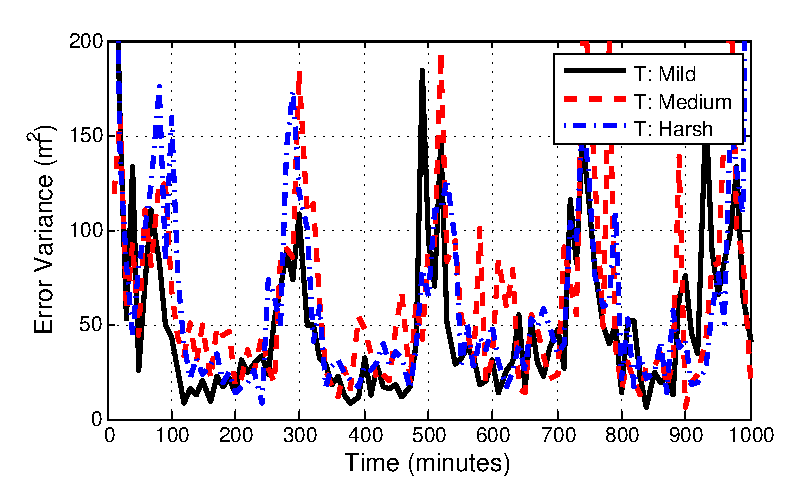
\includegraphics[width=\textwidth]{figures/localization_variance_novar}
  \captionof{figure}{\label{fig:loc_error_novar}Increased error variance for multi-agent localization assuming worst-case power }
\end{minipage}
}
\end{figure*}



Furthermore, the reduction in error variance when using VaRTOS does not come at the price of increased radio latency; the radio latency on the average will improve by using VaRTOS as well, as shown  for the case of harsh temperature profiles in the resulting optimal task performance in Table \ref{tab:loc_knobs}. The errors in energy consumption for this application are equivalent to those shown in Figure \ref{fig:app1_energy}, and thus we omit them here for the sake of brevity.


\begin{table}
\caption{\label{tab:loc_knobs}Task performance for multi-agent localization with and without VaRTOS with a harsh temperature profile}
\centering
\begin{tabular}{r|cccccccc}
\hline
Node ID & \#1 & \#2 & \#3 & \#4 & \#5 & \#6 & \#7 & \#8 \\ \hline
VaRTOS \# Avgs. & 35 & 34 & 31 & 30 & 28 & 27 & 23 & 10 \\
WC \# Avgs. & 6 & 6 & 6 & 6 & 6 & 6 & 6 & 6 \\
VaRTOS Freq (Hz) & 1.798  & 1.719 & 1.583 &1.527 & 1.459 & 1.380 & 1.176  & 0.525 \\
WC Freq (Hz) & 0.287 & 0.287 & 0.287 & 0.287 & 0.287 & 0.287 & 0.287 & 0.287 \\ \hline
\end{tabular}
\end{table}


%\begin{figure}
%\centering
%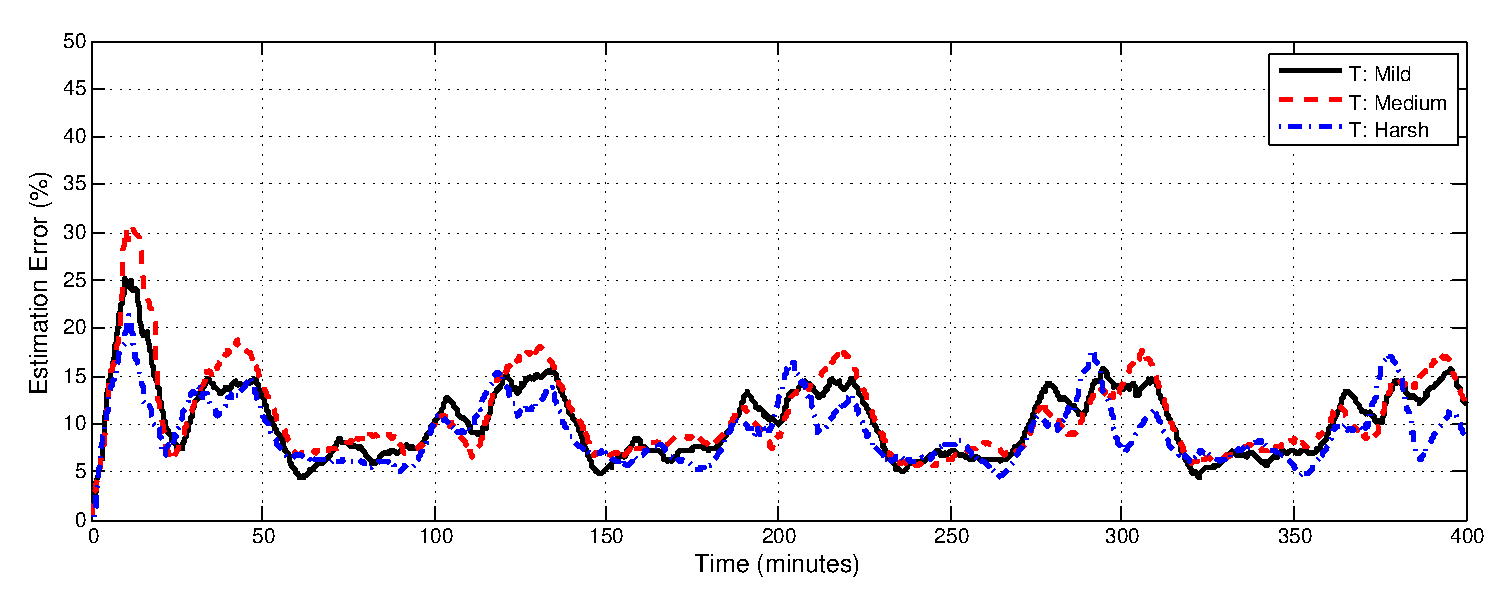
\includegraphics[width=0.5\textwidth]{figures/localization_var.eps}
%\caption{\label{fig:app1}App 1 dutycycle comparison}
%\end{figure}
%
%\begin{figure}
%\centering
%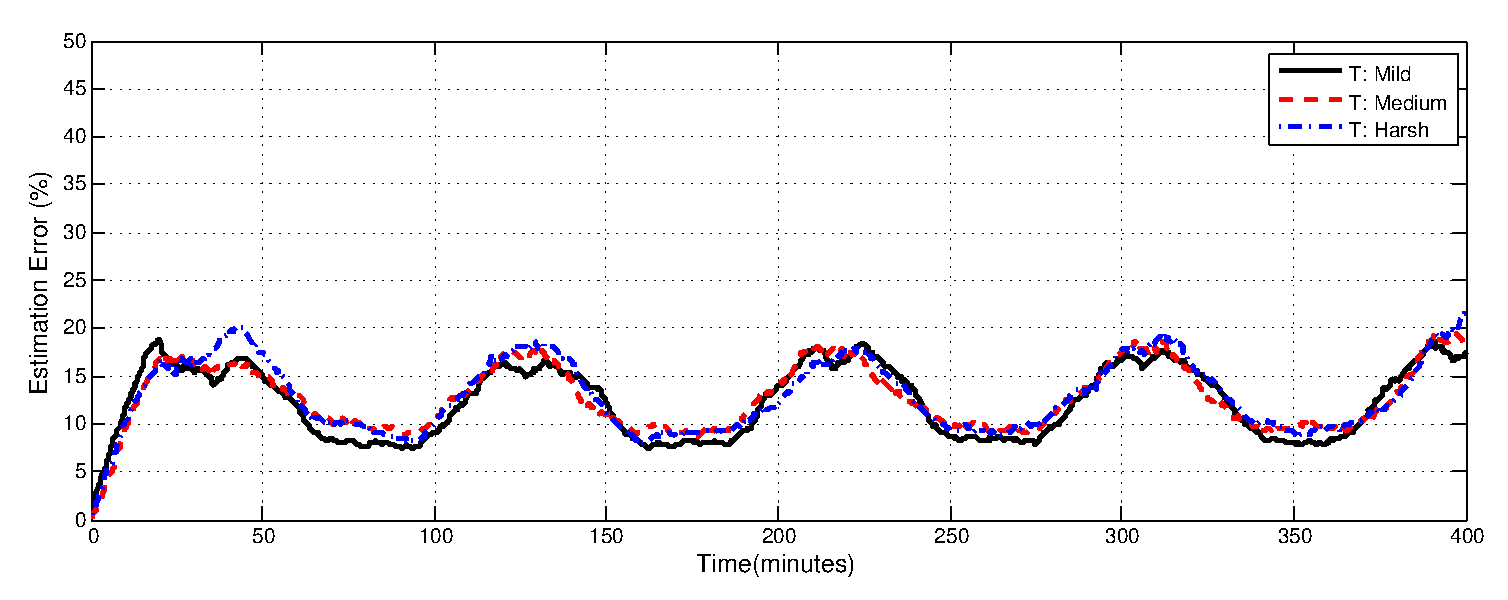
\includegraphics[width=0.5\textwidth]{figures/localization_novar.eps}
%\caption{\label{fig:app1}App 1 dutycycle comparison}
%\end{figure}
%

%\begin{figure}
%\centering
%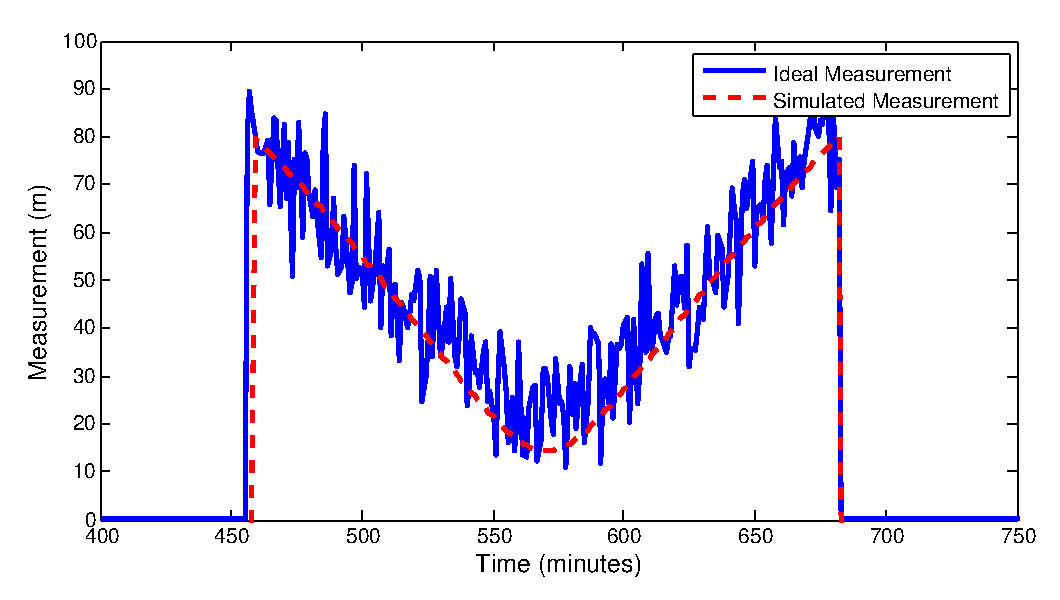
\includegraphics[width=0.5\textwidth]{figures/localization_stream_wc.eps}
%\caption{\label{fig:app1}App 1 dutycycle comparison}
%\end{figure}
%
%\begin{figure}
%\centering
%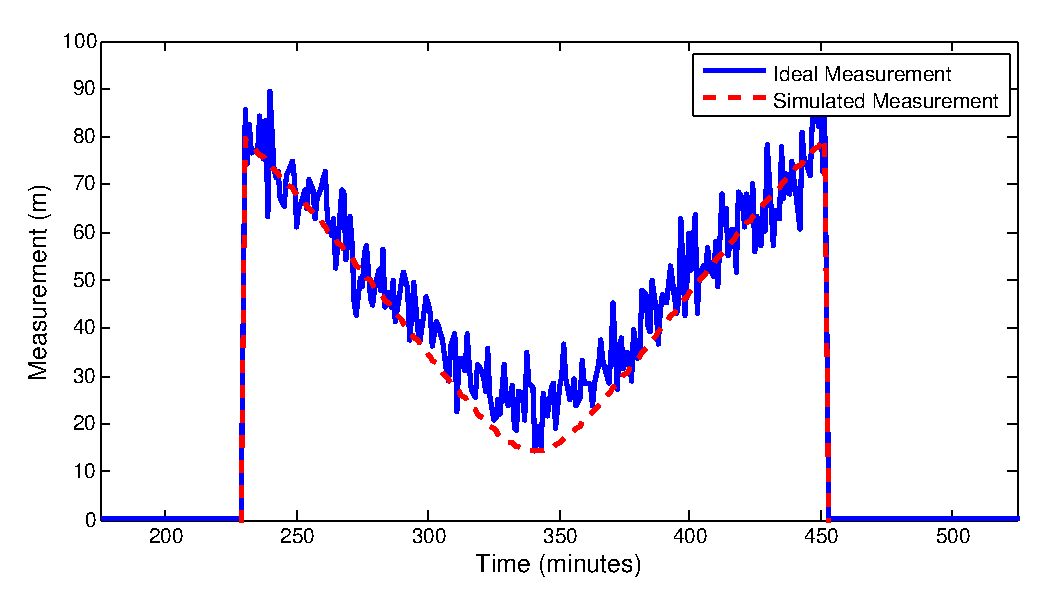
\includegraphics[width=0.5\textwidth]{figures/localization_stream_bc.eps}
%\caption{\label{fig:app1}App 1 dutycycle comparison}
%\end{figure}
%
%\begin{figure}
%\centering
%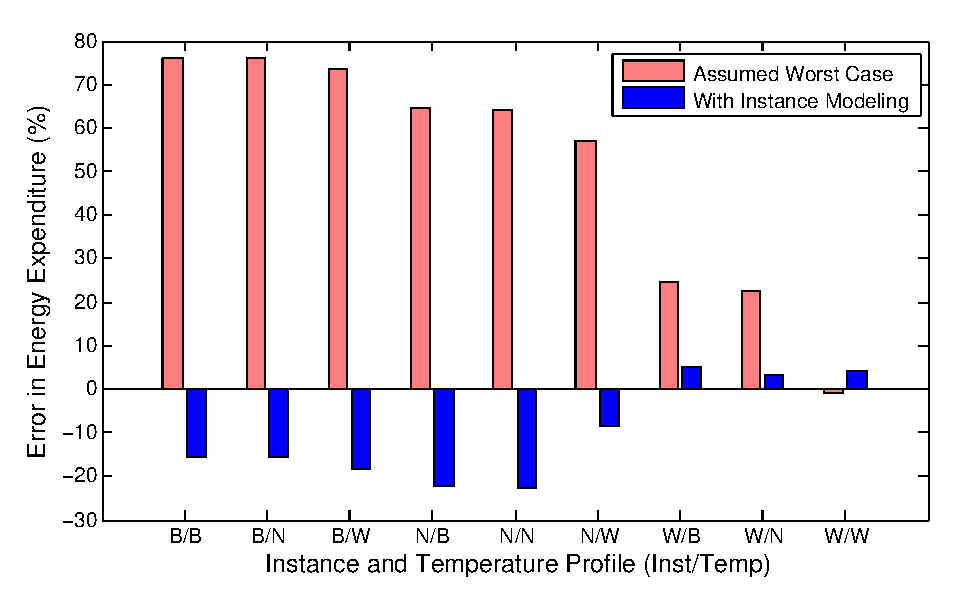
\includegraphics[width=0.5\textwidth]{figures/app3_energycomp.eps}
%\caption{\label{fig:app1}App 1 dutycycle comparison}
%\end{figure}



\subsection{Prediction-type Applications}
We now move away from wireless sensor network applications and look at systems of just a single node.  In particular, we consider an application where we would like to predict one quantity from another correlated but noisy quantity: in our case, we will predict velocity from position, perhaps again on a vehicle of some kind.  Here our tool of choice will be the Kalman filter, as it has become such a widely used tool even for resource-constrained applications. We are interested in calculating an estimate $\hat{v}$ of the velocity $v$ from measurements of the position, $y$, at various frequencies controlled again by a knob.  The system evolves according to the simple state space recursion: 

$$x_{k+1} = A_kx_k + B_ku_k~; ~~~~~ y_k = C_kx_k~;~~~~A_k= \begin{bmatrix}1 & \Delta t \\ 0 & 1\end{bmatrix}~~~~B_k = \begin{bmatrix} 0 & 1 \end{bmatrix}~~~~C_k = \begin{bmatrix} 1 & 0 \end{bmatrix}$$

For our case, $u_k$ will be a sinusoidal velocity input, and the goal is for $\hat{v}$ to track this input.  Intuitively, a faster sample rate for $y_k$ (meaning $\Delta t$ changes in $A$ as well) should give more accurate predictions of $\hat{v}$, because it is easier to predict states within the near future than it is to predict them in the distant future.  The Kalman recursion itself is omitted here, but we note that the Kalman gain and error covariance matrices (commonly denoted $K_{p,k}$ and $P_{k+1|k}$, respectively)  have to be modified on a per-instance basis in order to accommodate the varying sampling period, $\Delta t$. 


\begin{figure*}[t]
\centering
{\centering
\begin{minipage}{0.47\textwidth}
  \centering
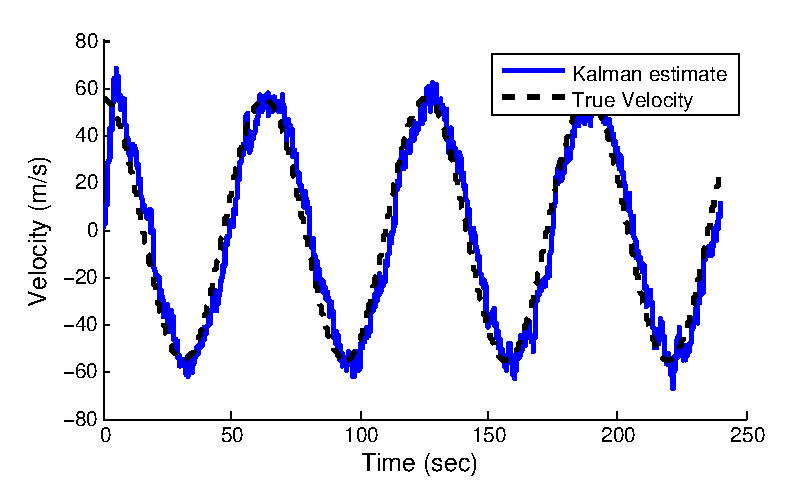
\includegraphics[width=\textwidth]{figures/kalman_example_vel}
  \captionof{figure}{\label{fig:kalman_ex}Kalman filter prediction of velocity from noisy position measurements}
\end{minipage}
\hspace{.04\textwidth}
\begin{minipage}{0.47\textwidth}
  \centering
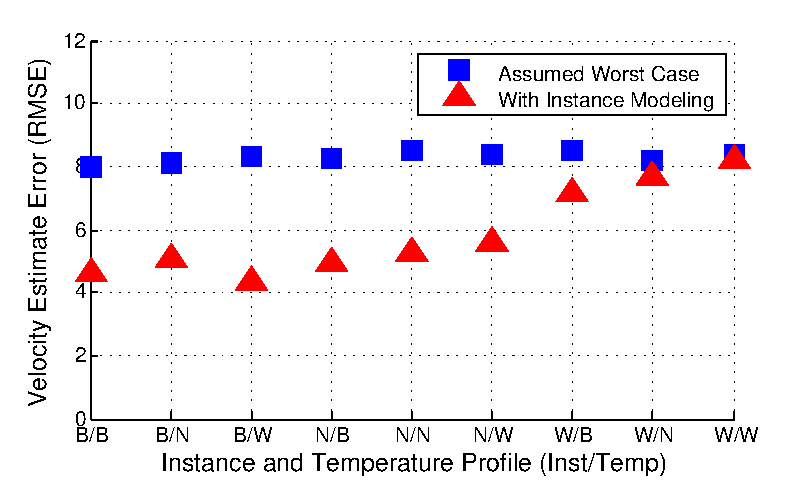
\includegraphics[width=\textwidth]{figures/kalman_results}
  \captionof{figure}{\label{fig:kalman_errors}Error (RMSE) in Kalman predictions when assuming worst case power consumption and when using VaRTOS }
\end{minipage}
}
\end{figure*}



Figure \ref{fig:kalman_ex} shows an example of the velocity input, $u_k$, as well as the estimated velocity as calculated by the Kalman filter on position $y_k$. Here the position readings are subjected to additive white Gaussian noise $\sim \normal(0, 50~m)$, and likewise the Kalman estimation of velocity contains some noise as well.  If we allow $\Delta t$ to assume values within the range $\Delta t \in [0.1~\text{s}, 10~\text{s}]$ by letting our knob vary as before, the quality of the estimate $\hat{v}$ will increase or decrease in accordance with energy surpluses and deficits, respectively.  Figure \ref{fig:kalman_errors} shows the error (RMSE) in estimating the velocity from noisy position measurements for systems assuming worst-case power and for those using instance-specific modeling with VaRTOS.  As before, the $x$-axis represents combinations of power instances (best-, nominal-, and worst-case) as well as temperature profiles (mild/best, medium/nominal, and harsh/worst). While the worst-case system has a constant error across all combinations, the VaRTOS results show a reduction in prediction error when additional work can be performed without sacrificing lifetime (i.e. those cases where weather and power instance result in a reduction in energy consumption over the worst-case). This improvement can be as much as 42.5\% in many cases. 


%
%\begin{figure}
%\centering
%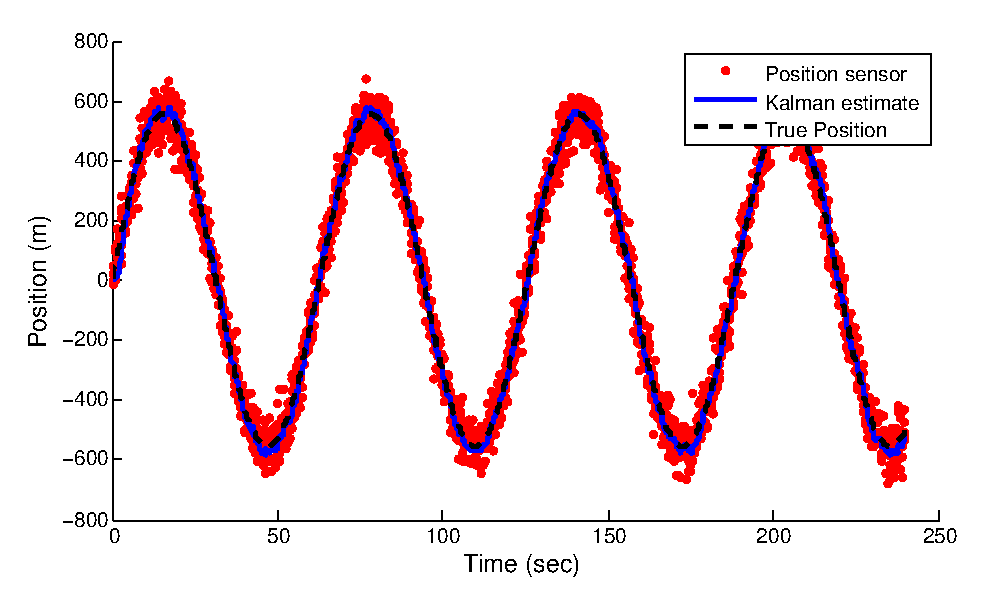
\includegraphics[width=0.5\textwidth]{figures/kalman_example_pos.eps}
%\caption{\label{fig:app1}App 1 dutycycle comparison}
%\end{figure}


\subsection{Block Processing Applications}

In some cases, a developer may have a number of signal processing (or similar) routines that would help to clean up or extract data from a particular signal.  In most cases, the total number of potential sensor processing blocks is likely to be small, and more importantly it is unlikely that each of these blocks will take the same time and thus the same power to complete.  In other words, the functions $\mathcal{K}_i$ that map knob values into duty cycles are no longer a very good fit, as the curve $k_i\rightarrow d_i$ is no longer linear.  As an example, consider a system with two sensor streams, each with 5 potential sensing blocks that all increase the quality of the application as a whole.  These tasks each take a distinct number of computer cycles to complete, as summarized in Table \ref{tab:blocks}.
\begin{table}
\caption{\label{tab:blocks}Processor cycle counts for a multi-block signal processing application}
\centering
\begin{tabular}{r|ccccc}
\hline
Block \# & 1 & 2 & 3 & 4 & 5 \\ \hline
Sensor 1 Block Cycles & 20000 & 5000 & 10000 & 25000 & 6000 \\
Sensor 2 Block Cycles & 14000 & 9000 & 15000 & 24000 & 8000 \\ \hline
\end{tabular}
\end{table}

%\begin{table}
%\caption{\label{tab:block_knobs}Optimal knob values (\# of blocks executed) for a multi-block signal processing application}
%\centering
%\begin{tabular}{r|ccccc}
%\hline
%Temperature & Power  & Sensor 1 & Sensor 1 & Sensor 2 & Sensor 2  \\
%& Instance & Worst-Case & VaRTOS & Worst-Case & VaRTOS \\ \hline
%Mild Weather & BC & 1 & 4 & 0 & 5\\
% & NC & 1 & 4  & 0 & 5\\
%& WC & 1 & 4  & 0 & 5\\
%Medium Weather & BC & 1 & 4  & 0 & 4\\
% & NC & 1 & 4  & 0 & 4\\
% & WC & 1 & 3  & 0 & 4\\
%Harsh Weather & BC & 1 & 1  & 0 & 2\\
% & NC & 1 & 1  & 0 & 2\\
% & WC & 1 & 0  & 0 & 1\\ \hline
%\end{tabular}
%\end{table}

\begin{figure}
\centering
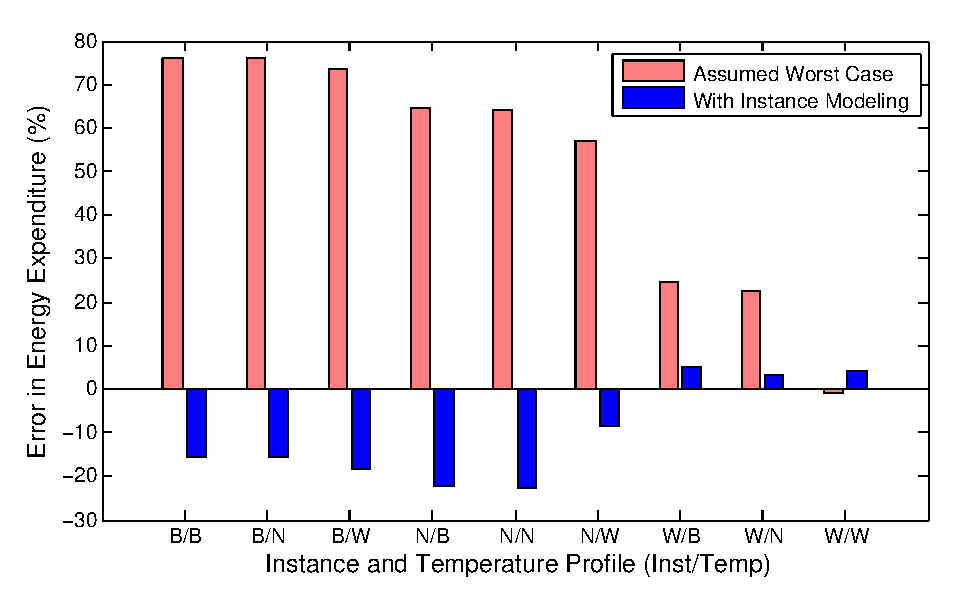
\includegraphics[width=0.6\textwidth]{figures/app3_energycomp}
\caption{\label{fig:app3_energycomp}Energy consumption errors for a mult-block signal processing application }
\end{figure}

The cycles  here have been arbitrarily chosen in part to show how VaRTOS responds to violations in architecture assumptions (linearity and granularity of task knobs).  If we try to schedule these two tasks using VaRTOS with $E = 12960~J$ and $L = 8760~h$ as before, the resulting errors in energy consumption will be those shown in Figure \ref{fig:app3_energycomp}.  In this case, the number of blocks executed using VaRTOS is on average 2.8 for sensor 1 and 3.5 for sensor 2 while worst-case power assumption resulted in 1 block between both sensors combined. In other words, while VaRTOS gives over a 64\% signal processing improvement in this application, the errors in energy expenditure are on average much larger than the errors shown in Figure \ref{fig:app1_energy}; indeed they would be even larger had our cycle counts shown in Table \ref{tab:blocks} varied even more or had the number of blocks been even fewer than 5.  While VaRTOS can help reduce energy errors to some extent in applications similar to this multi-block signal processing example, care should be taken to ensure that the assumptions made in Section \ref{sec:optimization} are not completely ignored. 





 % Paul
\section{Conclusion}
\label{sec:conclusion}
We developed an architecture for maximizing application quality while meeting lifetime and energy constraints in the face of power and temperature variation. We achieve this through application elasticity as defined by a \emph{knob}---a tunable variable that increases the quality of a given task at the expense of increased power consumption.  This knob serves to shape the utility curve of each task as well as offer a means by which the operating system can control the amount of active time and thus power given to individual tasks. We implemented online per-instance power modeling and task modeling in VaRTOS, a series of kernel extensions to the FreeRTOS operating system.  Our simulations using VaRTOS show that we can accurately meet a specified lifetime goal with less than 2\% error in most cases and less than 5\% error in the worst case, whereas had we assumed worst-case power consumption errors would range from 5\% to over 70\%.  We further demonstrated the ease with which a developer can adopt the VaRTOS architecture; very minimal user input is required, and the effects of these inputs can be tested using a graphical task modeling tool.  Finally, we presented case studies for multi-node localization applications using wireless sensor networks, estimation problems using Kalman filtering, and multi-block signal processing applications, illustrating how VaRTOS can increase application quality while maintaining lifetime requirements.  Knobs in VaRTOS represent flexible notions of elasticity---we make the assumption in this work that they have a linear relationship with computational time, but in general the only assumption required is that an increase in knob value will increase utility.  In other words, if more advanced modeling techniques are used, we can extend this notion of knobs to adapting many other system parameters, not just task frequency and duration. The VaRTOS architecture allows traditional, non-adaptive tasks to co-exist with adaptable tasks, and it is therefore suitable for a large class of applications where a notion of elasticity in quality exists.  Finally, all software developed in this project is open-source and can be found at https://github.com/nesl/vartos.  % Paul

% use section* for acknowledgement
\section*{Acknowledgment}
The authors would like to thank Supriyo Chakraborty for help with the initial problem formalization, Liangzhen Lai for valuable input regarding power variation models, and Puneet Gupta for help with the VarEMU project and additional prior work.  This material is based in part upon work supported by the NSF under
awards \# CCF-1029030, CNS-0905580,
CNS-0910706, and CNS-1143667.  Any opinions, findings and conclusions
or recommendations expressed
in this material are those of the author(s) and do not necessarily
reflect the views of the NSF.


%	REFERENCES		%
\bibliographystyle{ACM-Reference-Format-Journals}
\bibliography{bibliography,variability}

% History dates
%\received{May 2013}{TBD}{TBD}

% that's all folks
\end{document}


